\documentclass[12pt]{article}

% Page layout
\usepackage[a4paper, margin=1in]{geometry}

% Graphics and floats
\usepackage{graphicx}
\usepackage{tikz}
\usepackage{float}

% Title and spacing
\usepackage{titling}
\usepackage{setspace}

% Tables
\usepackage{booktabs}
\usepackage{array}
\usepackage{multirow}
\usepackage{longtable}
\usepackage{pdflscape}
\usepackage{tabularx}

% Text formatting
\usepackage{ragged2e}
\usepackage{parskip}
\usepackage{lipsum}
\usepackage{caption}

% Lists and symbols
\usepackage{enumitem, pifont}

% Code listings
\usepackage{listings}
\usepackage{xcolor}
\lstdefinestyle{mypython}{
    language=Python,
    backgroundcolor=\color{gray!10},
    basicstyle=\ttfamily\small,
    keywordstyle=\color{blue}\bfseries,
    commentstyle=\color{gray}\itshape,
    stringstyle=\color{teal},
    showstringspaces=false,
    numbers=left,
    numberstyle=\tiny\color{gray},
    stepnumber=1,
    numbersep=10pt,
    frame=single,
    breaklines=true,
    tabsize=4,
    captionpos=b
}

% Chemistry
\usepackage[version=4]{mhchem}    % for chemical formulas
\usepackage{chemfig}
\usepackage{chemmacros}
\chemsetup{modules={reactions}}   % Enable reaction schemes

% Math
\usepackage{amsmath, amssymb}

% Hyperlinks and references
\usepackage[colorlinks=true, linkcolor=blue, urlcolor=red, citecolor=green]{hyperref}
\usepackage{cleveref}  % optional but great for auto-formatting references

% Reference
\usepackage[utf8]{inputenc}

%\setcounter{tocdepth}{4}

\renewcommand{\arraystretch}{1.3}

\begin{document}

\begin{titlepage}
\centering
\vspace{1cm}

\Large \textbf{Computational studies on aromaticity, \\ Lewis acid-base adducts and applications using \\ Machine Learning methods}

\vspace{1cm}

{\large Report on work carried during } \\
{\large  the }

\vspace{0.5cm}

{\Large \textbf{Summer Internship 2025}}

\vspace{0.5cm}

{\large in}

\vspace{0.5cm}




\includegraphics[width=0.2\textwidth]{IISERK_Logo.png}



\vspace{1cm}

{\large \textit{Presented by}}

\vspace{0.3cm}

{\Large \textbf{Jeeva K}}

\vspace{0.3cm}

{\large 2\textsuperscript{nd} Year, 23MS234}
\\

{\large Indian Institute of Science Education and Research (IISER), Kolkata}

\vspace{1cm}


{\large \textit{Under supervision of:}}

\vspace{0.3cm}

{\Large \textbf{Dr. Debasis Koley}}

\vspace{0.3cm}

{\large Department of Chemical Sciences}
\\

{\large Indian Institute of Science Education and Research (IISER), Kolkata}

\end{titlepage}
\pagenumbering{roman}
\newpage
\begin{center}
    \section*{Declaration by the Student}
    \addcontentsline{toc}{section}{Declaration by the Student}
\end{center}

\vspace{1cm}

\justify
I, Jeeva K, hereby certify that I have performed all calculations for
this report titled \textbf{"Computational studies on aromaticity, Lewis acid-base adducts and applications using Machine Learning methods"}, based on my personal study and effort. This report is based on three research papers, which are duly acknowledged at the end. In addition to these references, I have conducted further independent work. All the calculations and analyses presented in this report were carried out independently and yielded consistent results.

\vspace{3cm}

\noindent
\begin{tabular}{@{}p{0.4\linewidth}@{}p{0.6\linewidth}@{}}
\textbf{Date:} 21/07/2025   \\[1.5ex]
\\
\\
\dotfill \\ &   \\[1.5ex]
\textbf{Place:} IISER Kolkata &  \hspace{3cm}\textbf{Jeeva K}\\[1.5ex]
& \hspace{1cm}Department of Chemical Sciences \\[1.55ex]
& Indian Institute of Science Education and Research  \\[1.5ex]
& \hspace{1cm} Kolkata, Mohanpur - 741246  \\[1.5ex]
& \hspace{2cm} West Bengal, India \\[1.5ex]
\end{tabular}


\vspace{2cm}
\noindent\dotfill

\newpage
\begin{center}
    \section*{Acknowledgments}
    \addcontentsline{toc}{section}{Acknowledgments}
\end{center}

\vspace{1cm}

\justify
I would like to express my sincere gratitude to my mentor, Prof. Debasis Koley, for his invaluable assistance throughout this project. His guidance at every step helped me learn many new things, making his presence during the internship incredibly valuable.

\vspace{1cm}

I would also like to thank Miss. Leya Elsa George and other CCMM members for their guidance throughout the project. I am also grateful to IISER Kolkata and CCMM lab for providing the necessary facilities for this work. Additionally, I extend my heartfelt thanks to my friends and parents for their unwavering support and encouragement.

\vspace{3cm}

\noindent
\begin{tabular}{@{}p{0.4\linewidth}@{}p{0.6\linewidth}@{}}
\textbf{Date:} 21/07/2025   \\[1.5ex]
\\
\\
\dotfill \\ &   \\[1.5ex]
\textbf{Place:} IISER Kolkata &  \hspace{3cm}\textbf{Jeeva K}\\[1.5ex]
& \hspace{1cm}Department of Chemical Sciences \\[1.55ex]
& Indian Institute of Science Education and Research  \\[1.5ex]
& \hspace{1cm} Kolkata, Mohanpur - 741246  \\[1.5ex]
& \hspace{2cm} West Bengal, India \\[1.5ex]
\end{tabular}

\vspace{2cm}

\noindent\dotfill



\newpage
\tableofcontents
\newpage
\begin{center}
\section*{Abstract}
\addcontentsline{toc}{section}{Abstract}
\end{center}
This report involves three computational studies that integrate quantum chemical calculations and machine learning to solve important challenges in molecular chemistry and chemical data analysis. In the first experiment, the concept of aromaticity is analyzed by calculating resonance energies using thermodynamic electronic energies of different homocyclic and heterocyclic hydrocarbons and ions using Gaussian 16. Geometry optimizations and frequency analyses were performed using semi-empirical AM1 methods, followed by Hartree-Fock single point energy calculations with the 3-21G(*) basis set to assess aromatic stabilization.

The second experiment investigates the binding interactions of various Lewis acid-base adducts involving Boron $\&$ aluminum hydrides and halides as acid and nitrogen $\&$ phosphorus containing bases. Computational methods identical to those in the first study were employed, with modifications in basis sets to evaluate electronic and steric effects. Key parameters such as HOMO-LUMO energies, vertical electron attachment energy, reorganization energy, and proton affinity were analyzed to determine relative acid-base strengths and reactivity.

The third experiment applies machine learning techniques to analyze a physicochemical dataset of red and white wines quality dataset. Using Interactive Python and Jupyter notebooks, the study covers data pre-processing, visualization, and supervised learning models to derive patterns and build predictive frameworks. All three experiments show the utility of computational chemistry and data science in understanding molecular properties and handling experimental datasets.




\newpage
\pagenumbering{arabic} 


%Experiment 1
\vspace*{\fill}
\begin{center}
    \section{Project: \MakeUppercase{\romannumeral 1} -  Quantitative Thermodynamic Descriptions of Aromaticity}\cite{quantitative_thermodynamic_aromaticity_2005}
    \label{project1}
    %\addcontentsline{toc}{section}{Quantitative Thermodynamic Descriptions of Aromaticity}
\end{center}
\vspace*{\fill}

\newpage
\newpage
\subsection{Introduction}
%\addcontentsline{toc}{subsection}{Introduction}
This study focuses on understanding the concept of aromaticity of organic compounds and verifying the aromaticity rules various homocyclic and heterocyclic hydrocarbons and hydrocarbon ions by finding their resonance energy, using computational calculations in \textit{Gaussian-16} software integrated with the \textit{GaussView-6} graphical interface.

The computational procedure involves constructing the organic molecule and Geometry Optimization+Frequency \textit{ (Opt+freq)} using \textit{ab-initio }semi-empirical AM1 calculation and followed by single point \textit{(sp)} energy calculations on the optimized structures using the Hartree-Fock method with the HF 3-21G(*) basis set.



%Theory
\subsection{Theory}
%\addcontentsline{toc}{subsection}{Theory}
\subsubsection{Aromaticity}
Aromatic Compounds are a crucial part of organic chemistry. The concept of Aromaticity is defined by Huckel's rule. For a molecule to be aromatic it should follow three rules.
\begin{itemize}[label=\ding{228}] 
    \item \textbf{Cyclic:} The molecule must be forming a closed loop.
    \item \textbf{Planar:} The molecule must have $sp^2$ hybridized orbitals, so that p-orbitals can overlap continuously.
    \item \textbf{Conjugation:} The ring must have alternate double bonds for conjugation of $\pi$ electrons;such that it is fully conjugated, allowing delocalization of $\pi$-electrons.
    \item \textbf{\boldmath$(4n + 2)\ \pi$-electrons:} The molecule must contain $(4n + 2) \pi-$ electrons in the conjugated system, where $n = (0, 1, 2,...).$
\end{itemize}

\begin{table}[!htp]
\centering
\footnotesize % or \footnotesize or \small
\renewcommand{\arraystretch}{1.5} % reduce row height a bit
\begin{tabular}{|>{\raggedright\arraybackslash}p{2.5cm}|>{\raggedright\arraybackslash}p{3.3cm}|>{\raggedright\arraybackslash}p{3.5cm}|>{\raggedright\arraybackslash}p{4cm}|}
\hline
\textbf{Property} & \textbf{Aromatic Compounds} & \textbf{Anti-Aromatic Compounds} & \textbf{Non-Aromatic Compounds} \\
\hline
Planarity & Planar & Planar & May or may not be planar \\
\hline
Conjugation & Fully conjugated (alternating $\pi$ bonds) & Fully conjugated & Not fully conjugated \\
\hline
Hückel's Rule & Follows $4n + 2$ $\pi$ electrons (n = 0, 1, 2, ...) & Follows $4n$ $\pi$ electrons (n = 1, 2, 3, ...) & Doesn’t follow Hückel’s rule \\
\hline
Stability & Highly stable due to delocalization of electrons & Highly unstable due to electron repulsion & No special stabilization \\
\hline
Delocalization of $\pi$ Electrons & Extensive and continuous delocalization & Delocalized but leads to instability & No continuous delocalization \\
\hline
Resonance Energy & Higher positive value & Higher negative value & Nearly equals to zero \\
\hline
\end{tabular}
\caption{Comparison between Aromatic, Anti-Aromatic, and Non-Aromatic Compounds}
\end{table}


\subsubsection{Resonance Energy}
The resonance energy explains the stability of aromatic compounds. We have used \textit{Isodesmic Isomerization reaction} for calculating the resonance energy of molecules. An Isodesmic Isomerization reaction is a hypothetical chemical reaction where the number and type of chemical bonds are the same on both sides of the equation. The isodesmic structures $(A  \&  B)$ shown in \Cref{fig:benzene_scheme},  of the desired molecules were constructed and their electronic energy  was computed, and the results were used to classify the compounds as aromatic, non-aromatic, or anti-aromatic.\\
%schemestart \chemfig{O*5(-=(-CH_3)-=--)} \arrow{->} \chemfig{O*5(--(=CH_2)-=--)} \schemestop

\begin{figure}[!htp]
\centering
\schemestart
  \chemname{\chemfig{*6(=-=-(-)=-)}}{Resonance Hybrid (\textbf{A})}
  \arrow{->}
  \chemname{\chemfig{*6(=-=-(=)--)}}{Isomer (\textbf{B})}
\schemestop
\caption{Example of Isodesmic Isomerization reaction.}
\label{fig:benzene_scheme}
\end{figure}



\subsubsection{Computational Calculation}
\textbf{Optimization + Frequency calculation: }This finds the molecular geometry with the lowest possible energy, which is the global minimum on the potential energy surface (PES) with only positive frequency values.

%This is used for finding the most stable geometry of the input molecule by adjusting the Potential Energy Surface (PES) and finding the global minima or the lowest energy structure to be the optimized geometry of the molecule.

\textbf{Single Point Energy Calculation:} This solves the Schrodinger equation using the approximation technique used by the given basis and finding the Total Electronic Energy of the input molecule at given geometry.

\textbf{Basis set }is a collection of mathematical functions which provide the tool to build the approximation to solve the Schrodinger equation  by representing the molecular orbitals as a linear combination of basis functions.

In computational chemistry, selecting an appropriate basis set is essential for balancing accuracy, time and computational cost. Geometry optimization and frequency calculations were performed using the semi-empirical AM1 method due to its efficiency for small and simple molecules. A more accurate single point energy calculation was then carried out using the Hartree-Fock method with the significantly higher-level 3-21G(*) basis set. All the calculations are done within seconds and the results are comparable with the higher basis-set calculation data.


%Observation and Results
\newpage
\subsection{Observation and Results}
%\addcontentsline{toc}{subsection}{Observation and Results}
The Resonance energy was calculated for the following molecules:\\
\textbf{6 homocyclic molecules:} Benzene, Naphthalene, cyclobutadiene, Cyclooctatetraene, Cycloheptatrienyl cation and Cycloheptatrienyl anion.\\
\textbf{3 heterocyclic molecules:} Furan, Pyridine, Thiophene.

The thermodynamic electronic energies of the isodesmic isomers of the given molecules were calculated. The resonance energy of each molecule was determined as the difference between the electronic energy of the isomer and that of the resonance hybrid, as shown below:

\begin{equation*}
E_{\text{Resonance}} = E_{B\;(Isomer)} - E_{A\;(Resonance Hybrid) }
\end{equation*}

The results are summarized in the tables \cref{Heterocyclic_table},\cref{Homocyclic_table}, \cref{Resonance_table}.\\
We can compare the Stability and Aromaticity of the molecules using resonance energy. As a whole, we can write the descending order of stability of organic compounds as:\\
\\
$
\text{Benzene} \gtrsim \text{Pyridine} > \text{Cycloheptatrienyl cation} > \text{Napthalene} > \text{Thiophene} > \text{Furan} > \text{Cyclooctatetraene} > \text{Cycloheptatrienyl anion} > \text{Cyclobutadiene}
$

\begin{table}[H]
\renewcommand{\arraystretch}{5}
\begin{tabular}{|>{\centering\arraybackslash}m{9.2cm}
                |>{\centering\arraybackslash}m{2cm}
                |>{\centering\arraybackslash}m{2cm}
                |>{\centering\arraybackslash}m{2cm}|}
\hline
\textbf{Resonance structures (A $\rightarrow$ B)} & \textbf{Energy of A (a.u.)} & \textbf{Energy of B (a.u.)} & \textbf{$\Delta E_{sp}$ (kcal/mol)} \\
\hline
\small \schemestart \chemfig{O*5(-=(-CH_3)-=--)} \arrow{->} \chemfig{O*5(--(=CH_2)-=--)} \schemestop & -266.16 & -266.15 & 11.23 \\
\hline
\small \schemestart \chemfig{N*6(=-=(-CH_3)-=--)} \arrow{->} \chemfig{N*6(=--(=CH_2)-=--)} \schemestop & -284.13 & -284.07 & 36.33 \\
\hline
\small \schemestart \chemfig{S*5(-=(-CH_3)-=--)} \arrow{->} \chemfig{S*5(--(=CH_2)-=--)} \schemestop & -587.41 & -587.38 & 15.56 \\
\hline

\end{tabular}
\caption{Resonance Energy calculation for heterocyclic compounds using their Isodesmic Isomerisation reaction}
\label{Heterocyclic_table}
\end{table}


\newpage

\begin{table}[!htp]
\renewcommand{\arraystretch}{6}
\begin{tabular}{|>{\centering\arraybackslash}m{8.8cm}
                |>{\centering\arraybackslash}m{2cm}
                |>{\centering\arraybackslash}m{2cm}
                |>{\centering\arraybackslash}m{2cm}|}
\hline
\textbf{Resonance structures (A $\rightarrow$ B)} & \textbf{Energy of A (a.u.)} & \textbf{Energy of B (a.u.)} & \textbf{$\Delta E_{sp}$ (kcal/mol)} \\
\hline
\tiny\schemestart\chemfig{*6(=-=(-CH_3)-=-=)} \arrow{->} \chemfig{*6(-=--(=CH_2)-=-=)} \schemestop & -268.23 & -268.17 & 37.66 \\
\hline
\tiny\schemestart \chemfig{*6(-=*6(-=-(-CH_3)=--)-=-=)} \arrow{->}  \chemfig{*6(-=*6(-=-(=CH_3)---)-=-=)} \schemestop & -420.03 & -419.99 & 25.31 \\
\hline
\tiny \schemestart \chemfig{*4(-=(-CH_3)-=-)} \arrow{->} \chemfig{*4(--(=CH_2)-=-)} \schemestop & -191.59 & -191.66 & -41.18 \\
\hline
\tiny \schemestart \chemfig{*8(=-=-=(-CH_3)-=-=)} \arrow{->} \chemfig{*8(=-=--(=CH_2)-=-=)} \schemestop & -344.62 & -344.62 & 0.55 \\
\hline
\tiny \schemestart \chemfig{*7(=-=(-CH_3)-\chemabove{C}{\oplus}-=--)}  \arrow{->}  \chemfig{*7(=--(=CH_3)-\chemabove{C}{\oplus}-=--)} \schemestop & -306.21 & -306.16 & 32.47 \\
\hline
\tiny \schemestart \chemfig{*7(=-=(-CH_3)-\chemabove{C}{\ominus}-=--)}  \arrow{->}  \chemfig{*7(=--(=CH_3)-\chemabove{C}{\ominus}-=--)} \schemestop & -306.33 & -306.36 & -19.28 \\
\hline
\end{tabular}
\caption{Resonance Energy calculation for homocyclic hydrocarbons and hydrocarbon ions using their Isodesmic Isomerisation reaction}
\label{Homocyclic_table}
\end{table}
\newpage
\renewcommand{\arraystretch}{1.5}
\begin{table}[H]
\centering
\begin{small}
\begin{tabular}{|>{\centering\arraybackslash}m{6cm}
                |>{\centering\arraybackslash}m{2.5cm}
                |>{\centering\arraybackslash}m{2cm}
                |>{\centering\arraybackslash}m{2cm}
                |>{\centering\arraybackslash}m{2.5cm}|}
\hline
\textbf{Structure} & \textbf{Number of $\pi$ electrons} & \textbf{Geometry} & \textbf{Resonance Energy (kcal/mol)} & \textbf{Aromaticity} \\
\hline
\tiny\chemname{\chemfig{**[0,360,dash pattern=on 2pt off 2pt]6(-=-=-=)}}{\small Benzene} \rule{0pt}{35pt} & 6 & Planar & 37.66 & Aromatic \\
\hline
\tiny\chemname{\chemfig{**[0,360,dash pattern=on 2pt off 2pt]6(-=**[0,360,dash pattern=on 2pt off 2pt]6(-=-=--)-=-=)}}{\small Naphthalene} \rule{0pt}{35pt} & 10 & Planar & 25.31 & Aromatic \\
\hline
\tiny\chemname{\chemfig{*4(-=-=-)}}{\small Cyclobutadiene} \rule{0pt}{35pt} & 4 & Planar & -41.18 & Anti-aromatic \\
\hline
\tiny\chemname{\chemfig{*8(-=-=-=-=-)}}{\small Cyclooctatetraene} \rule{0pt}{45pt} & 8 & Non-planar & 0.55 & Non-aromatic \\
\hline
\tiny\chemname{\chemfig{**[0,360,dash pattern=on 2pt off 2pt]7(=-=-\chemabove{C}{\oplus}-=--)}}{\small Cycloheptatrienyl cation} \rule{0pt}{40pt} & 6 & Planar & 32.47 & Aromatic \\
\hline
\tiny\chemname{\chemfig{*7(=-=-\chemabove{C}{\ominus}-=--)}}{\small Cycloheptatrienyl anion} \rule{0pt}{45pt} & 6 & Planar & -19.28 & Anti-aromatic \\
\hline
\tiny\chemname{\chemfig{O**[0,360,dash pattern=on 2pt off 2pt]5(-=-=--)}}{\small Furan} \rule{0pt}{45pt} & 6 & Planar & 11.23 & Aromatic \\
\hline
\tiny\chemname{\chemfig{S**[0,360,dash pattern=on 2pt off 2pt]5(-=-=--)}}{\small Thiophene} \rule{0pt}{35pt} & 6 & Planar & 15.56 & Aromatic \\
\hline
\tiny\chemname{\chemfig{N**[0,360,dash pattern=on 2pt off 2pt]6(=-=-=-)}}{\small Pyridine} \rule{0pt}{35pt} & 6 & Planar & 36.33 & Aromatic \\
\hline
\end{tabular}
\end{small}
\caption{Aromaticity in conjugated homocyclic and heterocyclic compounds }
\label{Resonance_table}
\end{table}




%Discussion
\newpage
\subsection{Conclusion and Discussion}
%\addcontentsline{toc}{subsection}{Discussion}


This study demonstrates the utility of computational chemistry in analyzing molecular structures and predicting chemical behavior. By applying electronic structure methods, researchers can gain insights into properties and bonding patterns that are often difficult to observe experimentally. The combination of molecular modeling and quantum mechanical calculations provides a framework for understanding chemical systems at the electronic level.

The use of isodesmic reactions in this experiment allowed for a practical and efficient approach to quantifying aromaticity. Since the method involves comparing structurally similar species with identical bonding patterns, it minimizes systematic errors and offers reliable energy differences. The calculations, although based on relatively small basis sets, produced meaningful results in a short computation time—showing strong agreement with theoretical expectations. This approach requires only the optimized geometry and electronic energy of two structures per molecule, making it suitable for a wide range of compounds. While this experiment focused on aromaticity, the same computational strategies are broadly applicable to various molecular systems as we are going to see in \cref{project2} .

In summary, this experiment highlights how computational tools like Gaussian and GaussView can model molecular structures, interpret bonding characteristics, and support chemical predictions. It reinforces the value of integrating theoretical methods with experimental insight to advance understanding in modern chemical research.\\

\noindent\dotfill



%Conclusion
%\subsection{Conclusion}
%\addcontentsline{toc}{subsection}{Conclusion}


%Experiment 2
\newpage
\vspace*{\fill}
\begin{center}
    \section{Project : \MakeUppercase{\romannumeral 2} - A Computational Analysis of Lewis Acids and Bases: Optimizing Electronic Properties and Reactivity}\cite{anderson_lewis_acid_base_2000}
    %\addcontentsline{toc}{section}{A Computational Analysis of Lewis Acids and Bases: Optimizing Electronic Properties and Reactivity}
    \label{project2section}
\end{center}
\vspace*{\fill}

\newpage
\subsection{Introduction}
%\addcontentsline{toc}{subsection}{Introduction}
The study investigates the relative strengths of various Lewis acids and bases by calculating the binding energies of their adducts and analyzing key factors influencing these interactions. Specifically, adducts formed between boron and aluminum based hydrides and halides as Lewis acids, nitrogen and phosphorus containing bases were examined using \textit{ab-initio} quantum mechanical methods. The same methodology and calculations from project 1 were performed with a different basis set Hartree-Fock HF 3-21G in Gaussian 16, with visualization in GaussView 6.

The relative acid and base strengths were evaluated through chemical hardness, determined from HOMO and LUMO energies. Additional parameters analyzed include vertical electron attachment energy, reorganization energy, proton affinity, and partial atomic charges on donor and acceptor atoms. Steric and electronic interactions were further explored by visualizing HOMO-LUMO orbital overlaps.

%Theory
\subsection{Theory}
%\addcontentsline{toc}{subsection}{Theory}
\subsubsection{Lewis acid and base}
\begin{itemize}
    \item \textbf{Lewis acid} is an electron pair acceptor. It possesses an empty orbital, often resulting from an electron-deficient central atom or a positive charge, which enables it to accept a pair of electrons from another species. This makes Lewis acids Electrophilic in nature, and they commonly have incomplete octets as in 13th Boron and Aluminum complexes. They have low energy LUMO orbital to accept electrons from HOMO of base.
    \item \textbf{Lewis base} is an electron pair donor. It has at least one lone pair of electrons available for donation, enabling it to form a coordinate covalent bond with a Lewis acid. Lewis bases are thus Nucleophilic, and typically feature atoms such as nitrogen, oxygen, or phosphorus with non-bonding electron pairs. They have high energy HOMO to donate electron to acids.
    \item \textbf{Acid–Base adduct} is a chemical compound formed when a Lewis base donates a lone pair of electrons to a Lewis acid, resulting in a coordinate covalent bond.
\end{itemize}

\subsubsection{Binding Energy}
Binding Energy ($\Delta E_{bind}$) is the energy difference between the adduct and the sum of the energies of the separate acid and base. For a gas-phase reaction between a Lewis acid and a
Lewis base, The binding energy is given by:

\[
\mathrm{A(g)} + \mathrm{:B(g)} \rightarrow \mathrm{A{:}B(g)}
\]
\[
\Delta E_{bind} = E_{A:B} - (E_{A} \;+ \; E_{B})
\]
\[
If \; \Delta E_{bind} < 0 	\Rightarrow Exothermic \;  and \;  Thermodynamically \; favourable
\]
\[
If \; \Delta E_{bind} > 0 	\Rightarrow Endothermic \;  and \;  Thermodynamically \; unfavourable
\]


\subsubsection{Factors Affecting Binding Energy}
A negative binding energy doesn't guarantee Lewis acid–base adduct formation, as factors like kinetics, sterics, and acid–base compatibility (e.g., hard–hard interactions) also influence binding. Here, we explore the key factors affecting adduct stability and binding energy.

\paragraph{i). Energies of HOMO and LUMO}~
\begin{itemize}
    \item A higher energy Highest Occupied Molecular Orbital(HOMO), closer to 0 eV or less negative means more willing to donate electrons. Therefore, a base with a high HOMO is considered a stronger Lewis base.
    \item A lower energy Lowest unoccupied Molecular Orbital (LUMO), more negative means more favorable to accept electrons. Therefore, an acid with a low LUMO is considered a stronger Lewis acid.
\end{itemize}
\paragraph{ii). Hardness of acid and base}
The Hardness is the concept which measures the strength of lewis acid and base and classify them as hard and soft. The hardness $(\eta)$ scale used here is Parr–Pearson Hardness (or Density Functional Theory-DFT Global Hardness) can be formulated as:
\[
\eta = \frac{E_{\text{LUMO}} - E_{\text{HOMO}}}2
\]
$Large \; \eta \Rightarrow $  Soft acid and base $\Rightarrow$ Species which resist change in electron density and less reactive. 

$Small \; \eta \Rightarrow $  Hard acid and base $\Rightarrow$ Species which more polarisable and more reactive.

\paragraph{iii). Reorganizational Energy of idealised acid: }
It is the energy required to change the geometry of the acid from trigonal planar to the idealized pyramidal structure. The geometry change happens when an acid interact with base during the formation of adduct.
\[
E_{reorg} = E_{planar} - E_{idealised \; pyramidal}
\]


\paragraph{iv). Reorganizational Energy of acid and base in adduct}
The base is removed from the adduct, and the energy of the acid in the geometry it adopts within the adduct, \( E_{AB}^{A} \), is calculated. The \textbf{reorganizational energy of the acid} is then given by \(  E_{AB}^{A} - E_0^A \), where \( E_0^A \) is the energy of the free acid at its own optimized geometry.

Similarly, the acid is removed from the adduct, and the energy of the base in the geometry it adopts within the adduct, \( E_{AB}^{B} \), is calculated. The \textbf{reorganizational energy of the base} is given by \( E_{AB}^{B} - E_0^B \), where \( E_0^B \) is the energy of the free base at its optimized geometry.

\paragraph{v). Vertical Electron Attachment Energy (VEAE) of acid}~
It is the energy change when an electron is added to a molecule without allowing the molecule to change its geometry. The geometry of acid remains same for both the structures, either planar or idealized pyramidal.
\[
E_{VEAE} = E_{pyamidal \; MX_3 } - E_{pyamidal \; MX_3^- } 
\]

\paragraph{vi). Proton affinity of base}~
It is a measure of the tendency of a base to accept a proton $(H^+)$ in the gas phase. It is proportional with the basicity of a molecule.

\[
\text{B (g)} + \text{H}^+ \rightarrow \text{BH}^+ \text{ (g)} \qquad \text{PA} = -\Delta H
\]
\[
\Delta H_{PA} = (\Delta H_{Base} +  \Delta H_{H^{+}}) -  \Delta H_{(Base-H)^{+}} 	\simeq \Delta H_{Base} -  \Delta H_{(Base-H)^{+}}
\]

\paragraph{vii). Charge transfer on adduct formation}~
It is the extent of net Mulliken charge transfer from base to acid in an adduct. It is the charge difference on the donor atom in its isolated state and in adduct. It can be formulated as:
\[
\Delta Q_{BA} = q_{isolated} \;-\; q_{adduct}
\]


\paragraph{viii). Change in the M–X bond distance in the acid}
\[
\Delta r_{MX} = \text{M-X bond length  of acid in adduct} - \text{M-X bond length  of free acid}
\]

\paragraph{ix). X–M–X bond angle in the acid of the adduct}
The \( \angle XMX\)  is the angle between the central and the substituent atoms. In a free acid with idealized pyramidal geometry, the angle is \( 109^\circ 50^{\prime\prime}\). But due to adduct formation, the \( \angle XMX\) changes and it can be observed in \cref{adduct_table}.


\paragraph{x). Electrostatic and steric interactions}~
Steric and electronic interactions refer to the repulsion caused by bulky groups surrounding the acceptor and donor centers of a Lewis acid or base. These interactions can hinder the close approach required for effective orbital overlap and reduce or prevent adduct formation. Even when the electronic properties like hardness, HOMO $\&$ LUMO energy levels favor adduct formation, steric hindrance can distort geometry and lower the stability or block the interaction entirely. This can be observed for 2,6-dimethylpyridine–\ce{BCl_3} adduct in \cref{adduct_table}, which despite involving one of the strongest Lewis acid-base pairs, exhibits lower binding energy compared to complexes such as \ce{NH_3}-\ce{AlCl_3} and 3,5-dimethylpyridine–\ce{BCl_3}. The reduced stability is attributed to steric hindrance from the methyl groups at the 2' and 6' positions of the pyridine ring, which prevents effective interaction with the Lewis acid.
\vspace{1em}

\textbf{Unit Conversion:}
\[
1 \;Hatree = 1 \;a.u.= 27.2114 \;eV= 627.509 \;kcal/mol = 2625.50\;kJ/mol
\]


\newpage
%Observation and Results
%\addcontentsline{toc}{subsection}{Observation and Results}
\subsection{Observation}
\label{project2}

\renewcommand{\arraystretch}{2}
\begin{table}[H]
\centering
\begin{tabular}{|>{\centering\arraybackslash}m{2cm}
                |>{\centering\arraybackslash}m{1.5cm}
                |>{\centering\arraybackslash}m{1.5cm}
                |>{\centering\arraybackslash}m{2cm}
                |>{\centering\arraybackslash}m{2cm}
                |>{\centering\arraybackslash}m{2cm}
                |>{\centering\arraybackslash}m{1.5cm}|}
\hline
\textbf{Molecule} & \textbf{$E_{HOMO}$ (eV)} & \textbf{$E_{LUMO}$ (eV)} & \textbf{Hardness (eV)} & \textbf{$\Delta E_{\mathrm{EA}^{a}}$ (kcal/mol)} & \textbf{$\Delta E_{\mathrm{reorg}}^{b}$ (kcal/mol)} & $Q_{AA}^{c}$ (statC) \\
\hline
\textbf{BH$_3$ }  & -12.87 & 1.15  & 7.01 & 8.29   & 24.37 & 0.03 \\
\hline
\textbf{BF$_3$  } & -16.96 & 0.47  & 8.72 & -5.65  & 46.18 & 1.19 \\
\hline
\textbf{BCl$_3$}  & -12.85 & -1.39 & 5.73 & -63.76 & 40.66 & 0.31 \\
\hline
\textbf{AlH$_3$ } & -11.28 & -0.02 & 5.63 & -13.91 & 20.69 & 0.76 \\
\hline
\textbf{AlCl$_3$} & -12.79 & -2.29 & 5.25 & -68.45 & 21.12 & 1.39 \\
\hline
\end{tabular}
\caption{Calculated Properties of the Idealized Pyramidal Boron and Aluminum
Hydrides and Halides using \textit{HF 3-21G basis set}}
\label{acid_table}
\end{table}

\renewcommand{\arraystretch}{1.5}
\begin{table}[H]
\centering
\begin{tabular}{|>{\centering\arraybackslash}m{4cm}
                |>{\centering\arraybackslash}m{1.5cm}
                |>{\centering\arraybackslash}m{1.5cm}
                |>{\centering\arraybackslash}m{2cm}
                |>{\centering\arraybackslash}m{2cm}
                |>{\centering\arraybackslash}m{1.5cm}|}
\hline
\textbf{Lewis base }& \textbf{$E_{\mathrm{HOMO}}$ (eV)} & \textbf{$E_{\mathrm{LUMO}}$ (eV)} &\textbf{ Hardness (eV)} &\textbf{ Proton Affinity (PA) (kcal/mol)} & $Q_{DA}^{d}$ (statC) \\
\hline
\textbf{NF$_3$ }& -15.01 & 6.02 & 10.52 & 126.24 & 0.65 \\
\hline
\textbf{PH$_3$ }& -10.36 & 4.93 & 7.64 & 184.27 & 0.09 \\
\hline
\textbf{NH$_3$ }& -10.59 & 7.49 & 9.04 & 226.94 & -0.88 \\
\hline
\textbf{Pyridine} & -9.69 & 3.54 & 6.61 & 241.22 & -0.67 \\
\hline
\textbf{3,5-Dimethylpyridine} & -9.13 & 3.56 & 6.34 & 246.06 & -0.68 \\
\hline
\textbf{N(CH$_3$)$_3$} & -9.08 & 6.92 & 8.00 & 248.03 & -0.68 \\
\hline
\textbf{2,6-Dimethylpyridine} & -9.08 & 3.62 & 6.35 & 250.04 & -0.75 \\
\hline
\end{tabular}
\caption{ Calculated Properties of the Lewis Bases using \textit{HF 3-21G basis set}}
\label{base_table}
\end{table}


$^{\mathrm{a}}$ Vertical electron attachment energy that occurs when an electron is added to the neutral \chemfig{MX_3} molecule at the idealized pyramidal geometry.\\
$^{\mathrm{b}}$ The re-organizational energy necessary to change the geometry of the
acid from trigonal planar to the idealized pyramidal structure.\\
$^{\mathrm{c}}$ The partial charge on the acceptor atom.\\
$^{\mathrm{d}}$ Partial charge on the donor atom \\

\newpage
\renewcommand{\arraystretch}{2}
\begin{table}[!htp]
\centering
\begin{tabular}{|>{\centering\arraybackslash}m{2.5cm}
                |>{\centering\arraybackslash}m{1.2cm}
                |>{\centering\arraybackslash}m{1cm}
                |>{\centering\arraybackslash}m{1cm}
                |>{\centering\arraybackslash}m{1.5cm}
                |>{\centering\arraybackslash}m{1.4cm}
                |>{\centering\arraybackslash}m{1.4cm}
                |>{\centering\arraybackslash}m{1cm}
                |>{\centering\arraybackslash}m{1cm}
                |>{\centering\arraybackslash}m{1cm}|}
\hline
\textbf{Adduct} & $\Delta BE^{a}$ (kcal mol$^{-1}$) & $r_{MN}^{b}$ (\AA) & $r_{MX}^{c}$ (\AA) & $\angle XMX^{d}$ ($^\circ$) & $E_\text{reorg acid}^{e}$ (kcal mol$^{-1}$) & $E_\text{reorg base}^{f}$ (kcal mol$^{-1}$) & $\Delta Q_{BA}^{g}$ & $\Delta Q_{DA}^{h}$ & $Q_{AA}^{i}$ \\
\hline
H$_3$N:AlCl$_3$ & -66.98 & 1.98 & 0.04 & 116.50 & 6.61 & 0.54 & 0.25 & -1.01 & 1.40 \\
\hline
H$_3$N:BCl$_3$ & -49.14 & 1.63 & 0.10 & 113.50 & 24.98 & 0.40 & 0.36 & -0.90 & 0.27 \\
\hline
H$_3$N:AlH$_3$ & -42.88 & 2.05 & 0.02 & 116.86 & 5.42 & 0.33 & 0.19 & -0.96 & 0.74 \\
\hline
H$_3$N:BF$_3$ & -42.09 & 1.69 & 0.05 & 114.13 & 24.11 & 0.20 & 0.20 & -0.98 & 1.19 \\
\hline
H$_3$N:BH$_3$ & -35.65 & 1.71 & 0.02 & 113.95 & 13.59 & 0.22 & 0.26 & -0.86 & 0.00 \\
\hline
H$_3$P:AlCl$_3$ & -27.27 & 2.54 & 0.04 & 116.74 & 6.11 & 2.56 & 0.14 & -0.04 & 1.43 \\
\hline
H$_3$P:AlH$_3$ & -12.69 & 2.72 & 0.01 & 118.67 & 2.23 & 0.85 & 0.05 & 0.00 & 0.80 \\
\hline
H$_3$P:BH$_3$ & -8.39 & 2.21 & 0.01 & 116.80 & 6.96 & 1.07 & 0.27 & 0.24 & -0.18 \\
\hline
H$_3$P:BCl$_3$ & -7.73 & 2.06 & 0.10 & 113.85 & 23.76 & 4.33 & 0.66 & 0.49 & -0.16 \\
\hline
H$_3$P:BF$_3$ & -5.70 & 3.03 & 0.00 & 119.74 & 0.90 & 0.17 & 0.01 & 0.02 & 1.20 \\
\hline
3,5-Dimethyl-pyridine:BCl$_3$ & -47.92 & 1.61 & 0.12 & 111.07 & 33.72 & 0.65 & 0.36 & -0.96 & 0.35 \\
\hline
pyridine:BCl$_3$ & -46.68 & 1.61 & 0.12 & 111.24 & 33.01 & 0.69 & 0.35 & -0.94 & 0.35 \\
\hline
2,6-Dimethyl-pyridine:BCl$_3$ & -28.66 & 1.62 & 0.13 & 111.49 & 42.20 & 10.83 & -0.36 & -1.00 & 0.35 \\
\hline
\end{tabular}
\caption{Calculated properties of Ammonia and Phosphine adducts of Lewis acid using \textit{HF 3-21G basis set.}}
\label{adduct_table}
\end{table}


$^{\mathrm{a}}$ Binding energy. \\
$^{\mathrm{b}}$ Donor atom-acceptor atom bond distance in the adduct.\\
$^{\mathrm{c}}$ Change in the M-X bond distance in the acid of the adduct.\\
$^{\mathrm{d}}$ Value of the X-M-X bond angle in the acid of the adduct.\\
$^{\mathrm{e}}$ Re-organizational energy of the acid upon adduct formation as a result of a change in the structure.\\
$^{\mathrm{f}}$ Re-organizational energy of the acid upon adduct formation as a result of a change in the structure.\\
$^{\mathrm{g}}$ Net Mulliken Charge transfer from the base to the acid upon adduct formation.\\
$^{\mathrm{h}}$ Charge on the donor atom of the base in the adduct.\\
$^{\mathrm{i}}$ Charge on the acceptor atom of the acid in the adduct.\\


%Figures

%\newpage
% For Printout
% \begin{figure}[htp]
%     \centering
%     \fbox{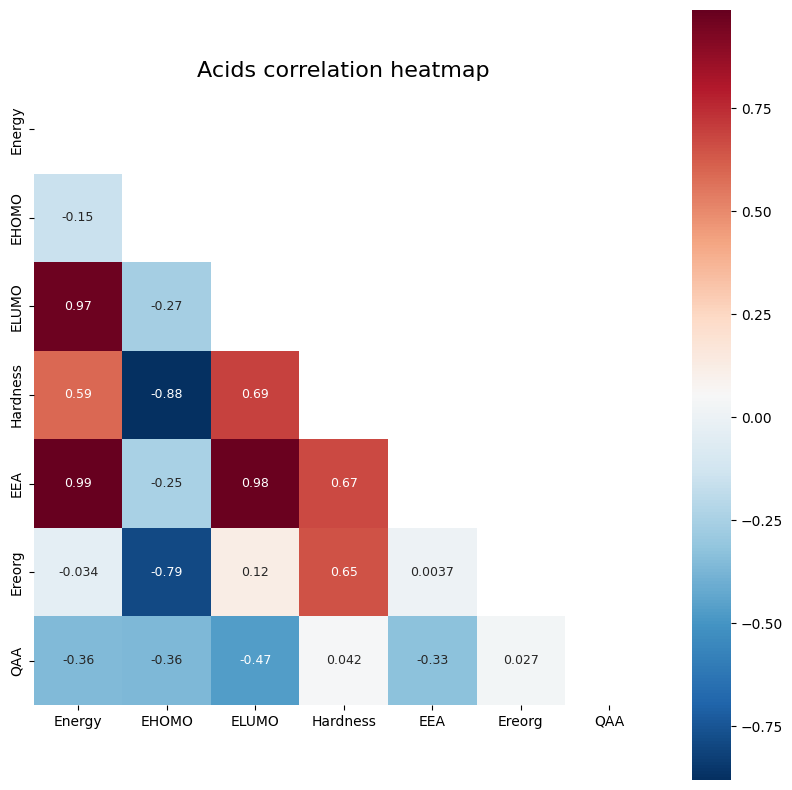
\includegraphics[width=16cm, height=7.5cm]{Acid_Base/images/acid_heatmap.png}}
%     \caption{Heatmap with corelation coefficient showing relation between different quantitative variables of Acids}
%     \label{fig:Acid_heatmap}
% \end{figure}
% \begin{figure}[htp]
%     \centering
%     \fbox{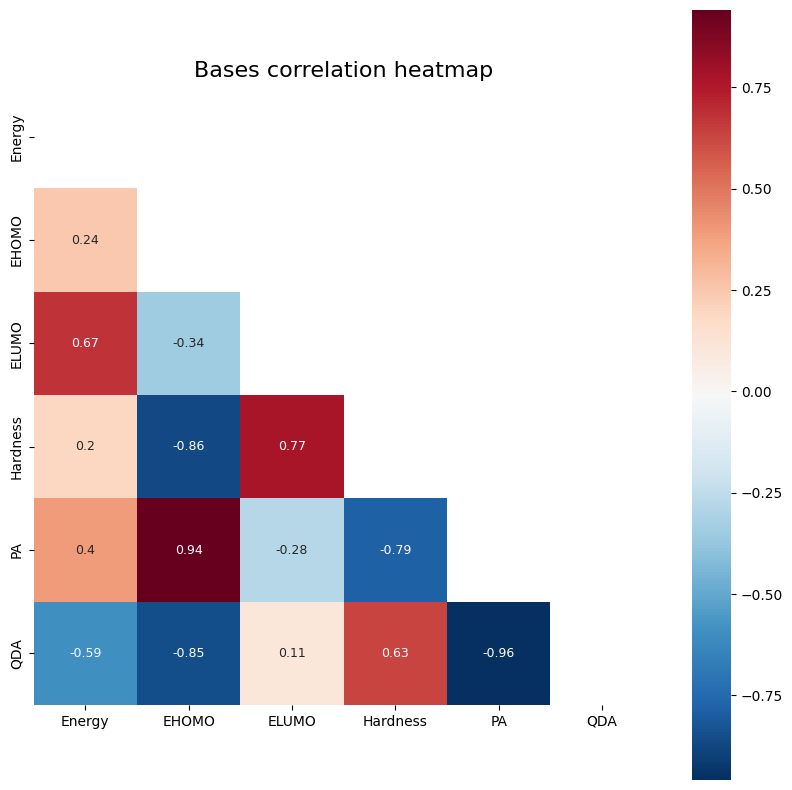
\includegraphics[width=16cm, height=7.5cm]{Acid_Base/images/base_heatmap.png}}
%     \caption{Heatmap with corelation coefficient showing relation between different quantitative variables of Bases}
%     \label{fig:Base_heatmap}
% \end{figure}

% For online PDF
\newpage
\begin{figure}[H]
    \centering
    \fbox{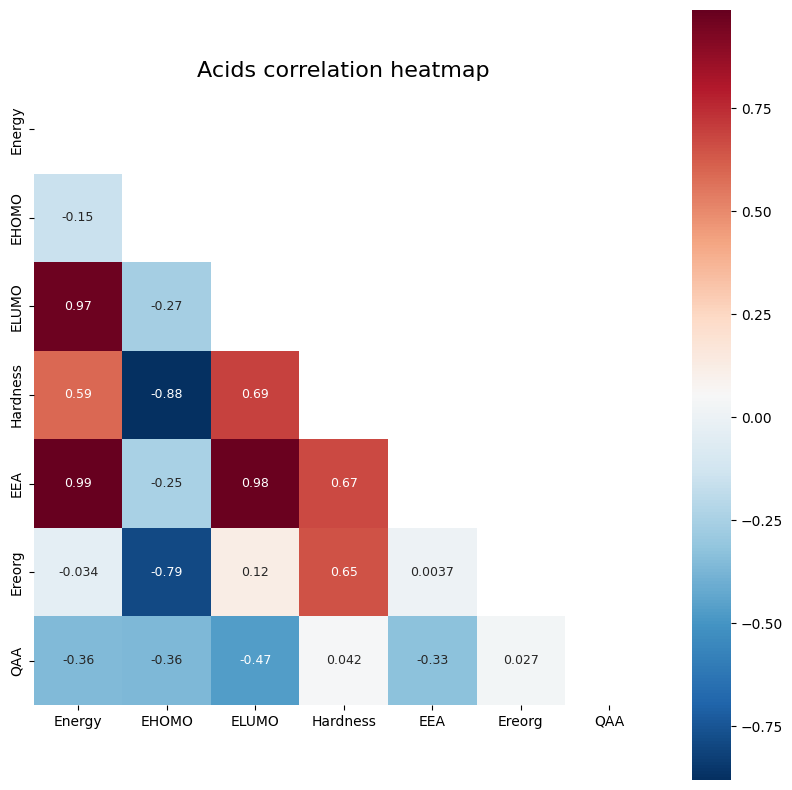
\includegraphics[width=\textwidth]{Acid_Base/images/acid_heatmap.png}}
    \caption{Heatmap with corelation coefficient showing relation between different quantitative variables of Acids}
    \label{fig:Acid_heatmap}
\end{figure}

\newpage
\begin{figure}[H]
    \centering
    \fbox{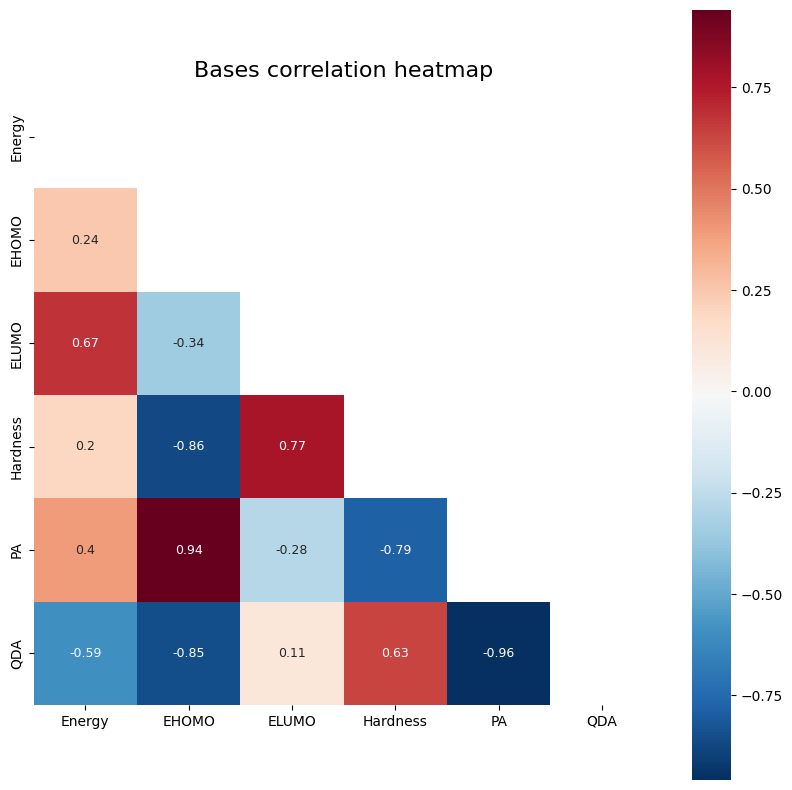
\includegraphics[width=\textwidth]{Acid_Base/images/base_heatmap.png}}
    \caption{Heatmap with corelation coefficient showing relation between different quantitative variables of Bases}
    \label{fig:Base_heatmap}
\end{figure}

\begin{figure}[H]
    \centering
    % First image
    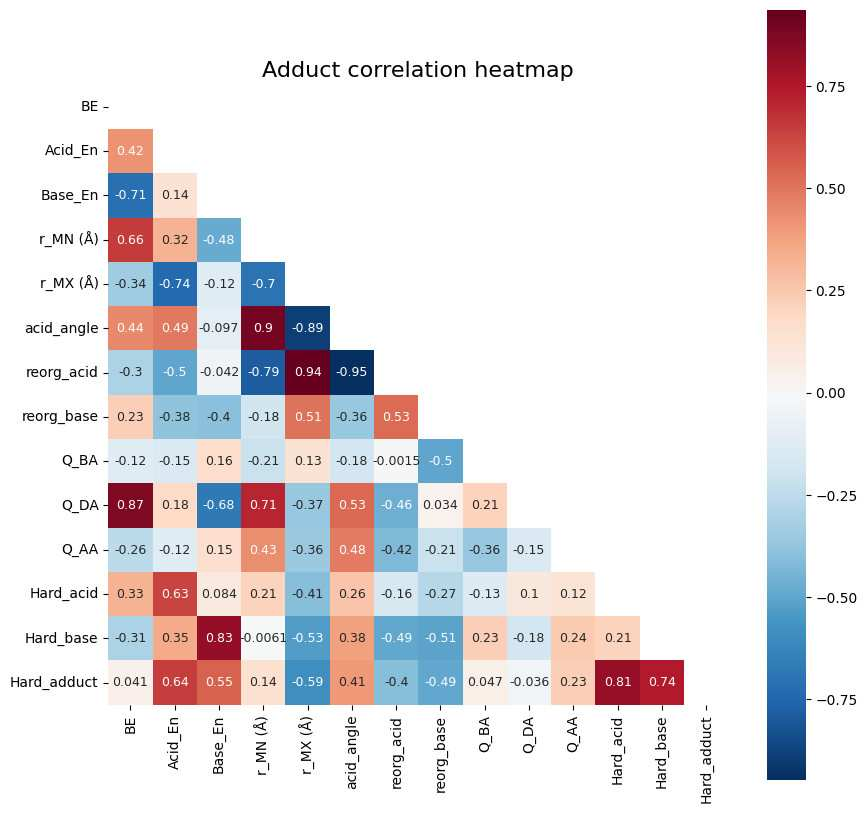
\includegraphics[width=0.9\linewidth]{Acid_Base/images/adduct_heatmap.jpeg}
    \caption{Heatmap with corelation coefficient showing relation between different quantitative variables of Acid-Base adducts}
    \label{fig:adduct-heatmap}

    \vspace{1em} % Vertical space between images

    % Side-by-side images
    \begin{minipage}[b]{0.48\linewidth}
        \centering
        \fbox{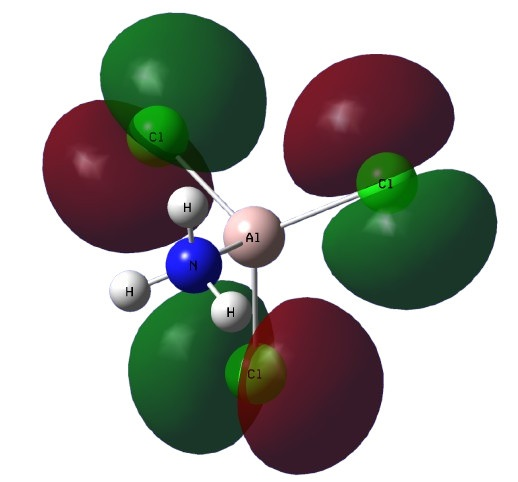
\includegraphics[width=\linewidth]{Acid_Base/images/NH3_AlCl3_homo.jpeg}
        \caption*{(a) $NH_3-AlCl_3$ adduct HOMO}}
    \end{minipage}
    \hfill
    \begin{minipage}[b]{0.48\linewidth}
        \centering
        \fbox{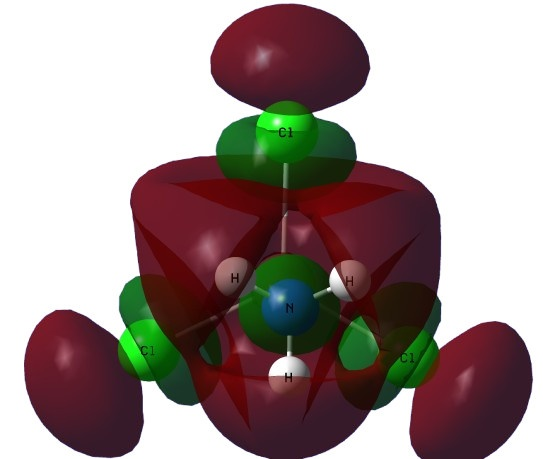
\includegraphics[width=\linewidth]{Acid_Base/images/NH3_AlCl3_lumo.jpeg}
        \caption*{(b) $NH_3-AlCl_3$ adduct LUMO}}
    \end{minipage}
    %\caption{Side-by-side comparison of two figures.}
    %\label{fig:side-by-side}
\end{figure}

\newpage
%Discussion
\subsection{Results}
%\addcontentsline{toc}{subsection}{Discussion}
\subsubsection{Strength of acid, base and adducts}
From the observation of hardness value of acids from \cref{acid_table}, the descending order of the strength of acid can be given as:
\[AlCl{_3} > AlH_3 > BCl_3 > BH_3 > BF_3 \]
From the observation of hardness value of acids from \cref{base_table}, the descending order of the strength of base can be given as:
\[ 3,5-dimethylpyridine \simeq 2,6-dimethylpyridine > pyridine > PH_3 > N(CH_3)_3 > NH_3 > NF_3 \]
From observation of the binding energy value of the Lewis acid ammonia and phosphorus adducts of \cref{adduct_table}, the descending order of the strength of the adducts can be given as:
\begin{align*}
& NH_3\text{–}AlCl_3 > NH_3\text{–}BCl_3 > 3,5\text{-dimethylpyridine–}BCl_3 > \text{pyridine–}BCl_3 > \\
& NH_3\text{–}AlH_3 > NH_3\text{–}BF_3 > NH_3\text{–}BH_3 > PH_3\text{–}AlCl_3 > \\
& 2,6\text{-dimethylpyridine–}BCl_3 > PH_3\text{–}AlH_3 > PH_3\text{–}BH_3 > PH_3\text{–}BCl_3 > PH_3\text{–}BF_3
\end{align*}

\subsubsection{Correlation Heatmap}
A correlation heatmap is a data visualization technique that uses color to represent Pearson's correlation coefficient (r) in a 2D matrix. The value of the correlation coefficient ranges from 1 to -1.
\begin{align*}
r &= +1 \Rightarrow \text{Perfect positive linear correlation (all points lie exactly on a line with positive slope)} \\
r &\in (0, 1) \Rightarrow \text{Weak to strong positive linear correlation with deviations from straight line} \\
r &= 0 \Rightarrow \text{No linear or non-linear correlation} \\
r &\in (-1, 0) \Rightarrow \text{Weak to strong negative linear correlation with deviations from straight line} \\
r &= -1 \Rightarrow \text{Perfect negative linear correlation (all points lie exactly on a line with negative slope)}
\end{align*}


From the acid correlation heat map shown in \cref{fig:Acid_heatmap}, we can visualize the relationship between different factors affecting the hardness of acid. We can write the following conclusion from it.
\[
Strength \propto \frac{1}{Hardness} \propto \frac{1}{E_{LUMO}} \propto E_{HOMO}  \propto \frac{1}{E_{EA}} \propto \frac{1}{E_{reorg}} \propto \frac{1}{Energy}
\]

From the base correlation heat map shown in \cref{fig:Base_heatmap}, we can visualize the relationship between different factors affecting the hardness of base. We can write the following conclusion from it.
\[
Strength \propto \frac{1}{Hardness} \propto \frac{1}{E_{LUMO}} \propto E_{HOMO} \propto \Delta E_{PA}  \propto \frac{1}{Q_{DA}}
\]

\newpage
From the adduct correlation heat map shown in \cref{fig:adduct-heatmap}, we can visualize the relationship between different factors that affect the hardness of the Ammonia and Phosphine adducts of Lewis acid. From this we can draw the following conclusion.
\[
\Delta E_{bind} \propto \frac{1}{E_{base}} \propto Q_{DA} \propto r_{MN} \propto \angle XMX \propto E_{acid}
\]
\[
r_{MX} \propto \Delta E_{reorg \; acid} \propto \frac{1}{\angle XMX}
\]
\[
r_{MN} \propto \angle XMX \propto Q_{DA} \propto \frac{1}{\Delta E_{reorg \; base}} \propto \frac{1}{r_{MX}}
\]


%Conclusion
\subsection{Discussion and Conclusion}
%\addcontentsline{toc}{subsection}{Conclusion}
This study demonstrated that \textit{ab-initio single point Hatree Fock HF/3-21G} calculations effectively capture trends in Lewis acid-base adducts binding energies and related electronic properties. The Key parameters such as $E_{LUMO}, E_{HOMO} ,$ hardness, and proton affinity were consistent with higher-level data from literature (Anderson, 2000), confirming the method’s reliability for qualitative analysis.

Overall, this work provides a foundation for future studies involving more complex systems or higher levels of theory. The ability to predict and interpret acid-base behavior computationally is a powerful tool for guiding experimental design and advancing theoretical understanding in coordination chemistry, catalysis, and materials science.\\


\noindent\dotfill

\newpage


\newpage
\vspace*{\fill}
\begin{center}
    \section{Project: \MakeUppercase{\romannumeral 3} - Machine Learning for Chemists: Using Python Notebooks for Visualization, Data Processing, Analysis, and Modeling of wine dataset}\cite{lafuente_gentle_ml_2021}
    %\addcontentsline{toc}{section}{Machine Learning for Chemists: Using Python Notebooks for Visualization, Data Processing, Analysis, and Modeling of wine dataset}
\end{center}
\vspace*{\fill}

\newpage
\newpage
\subsection{Introduction}

The integration of automation and Internet of Things (IoT) technologies in laboratories has revolutionized chemical research by enabling the collection of large, complex datasets involving multiple physicochemical variables. With this shift, data analysis and scientific computing—particularly machine learning—have become vital tools for extracting insights and building predictive models.

This study focuses on developing foundational machine learning skills using Python, with an emphasis on real-world data analysis. Using interactive platforms such as Jupyter Notebook and Google Colab, we explored a dataset comprising the physicochemical properties of red and white wines. We acquired basic knowledge of essential Python libraries used in machine learning and applied various techniques for data visualization, pre-processing, analysis, and modeling of the wine dataset.

% \subsection{Theory}
% This section explains the foundational concepts used

\subsection{Basic Definitions}
\begin{itemize}
    \item \textbf{Dataset:} It is a structured collection of data organized in tabular form, where each row represents a single observation or record, and each column corresponds to a specific variable or feature.
    \item \textbf{Dataframe:} It is a two-dimensional, size-mutable, and heterogeneous data structure in Python provided by the Pandas library
\end{itemize}

\renewcommand{\arraystretch}{1}
\begin{table}[!htp]
\centering
\caption{Dataset Description from Wine Dataset Containing Sample Quantities of Each Wine Type, Wine Physicochemical Attributes, and Their Corresponding Units}
\begin{tabular}{|l|l|l|}
\multicolumn{3}{c}{\textbf{input variables}} \\
\hline
\textbf{No.} & \textbf{Features} & \textbf{Units} \\
\hline
1 & fixed acidity & g(tartaric acid)/dm$^3$ \\
2 & volatile acidity & g(acetic acid)/dm$^3$ \\
3 & citric acid & g/dm$^3$ \\
4 & residual sugar & g/dm$^3$ \\
5 & chlorides & g(sodium chloride)/dm$^3$ \\
6 & free sulfur dioxide & mg/dm$^3$ \\
7 & total sulfur dioxide & mg/dm$^3$ \\
8 & density & g/cm$^3$ \\
9 & pH & -- \\
10 & sulfates & g(potassium sulfate)/dm$^3$ \\
11 & alcohol & vol \% \\
\hline
\multicolumn{3}{c}{} \\
\multicolumn{3}{c}{\textbf{output variable}} \\
\hline
\textbf{No.} & \textbf{Labels }& \textbf{Units }\\
\hline
12 & quality & -- \\
\hline
\multicolumn{3}{c}{} \\
\hline
\textbf{Samples} & 1599 & red wine \\
        & 4898 & white wine \\
\hline
\end{tabular}
\label{features_table}
\end{table}

\begin{table}[htbp]
\centering
\caption{Python Libraries Used in the Notebooks to Analyze and Plot the Data}
\begin{tabular}{|l|p{4.5cm}|p{5cm}|}
\hline
\textbf{Library Name} & \textbf{Description} & \textbf{Website} \\
\hline
Matplotlib & Plotting tools & \url{https://matplotlib.org/} \\
\hline
NumPy & Linear algebra and fast math library & \url{https://numpy.org/} \\
\hline
Pandas & Handling and preprocessing of large data sets & \url{https://pandas.pydata.org/} \\
\hline
Pingouin & Common statistical tests & \url{https://pingouin-stats.org/} \\
\hline
Seaborn & Advanced plotting functions & \url{https://seaborn.pydata.org/} \\
\hline
Plotly & Interactive plots and advanced plotting functions & \url{https://plotly.com/python/} \\
\hline
Scikit-Learn & Scientific computing and machine learning tools & \url{https://scikit-learn.org/} \\
\hline
\end{tabular}
\label{library_table}
\end{table}


As shown in \cref{features_table}, both the red and white wine datasets contain 12 variables, out of which 11 input variables are derived from the chemical analysis of wine, and one output variable "quality" which reflects the effectiveness of the wine based on these inputs.

We utilized all the Python libraries listed in \cref{library_table}, along with Ipywidgets, to create interactive and advanced 3D visualizations.

\subsubsection{Importing wine datasets}
\begin{lstlisting} [style=mypython]
red_df = pd.read_csv("https://archive.ics.uci.edu/ml/machine-learning-databases/wine-quality/winequality-red.csv", delimiter=";")
white_df = pd.read_csv("https://archive.ics.uci.edu/ml/machine-learning-databases/wine-quality/winequality-white.csv", delimiter=";")
\end{lstlisting}


\newpage

\subsection{Data Visualization using statistical plots}

\subsubsection{Histogram}

\begin{lstlisting}[style=mypython]
sns.set()
red_df.hist(figsize=(12,12), color='red')
plt.show()
\end{lstlisting}


\begin{figure}[H]
    \centering
    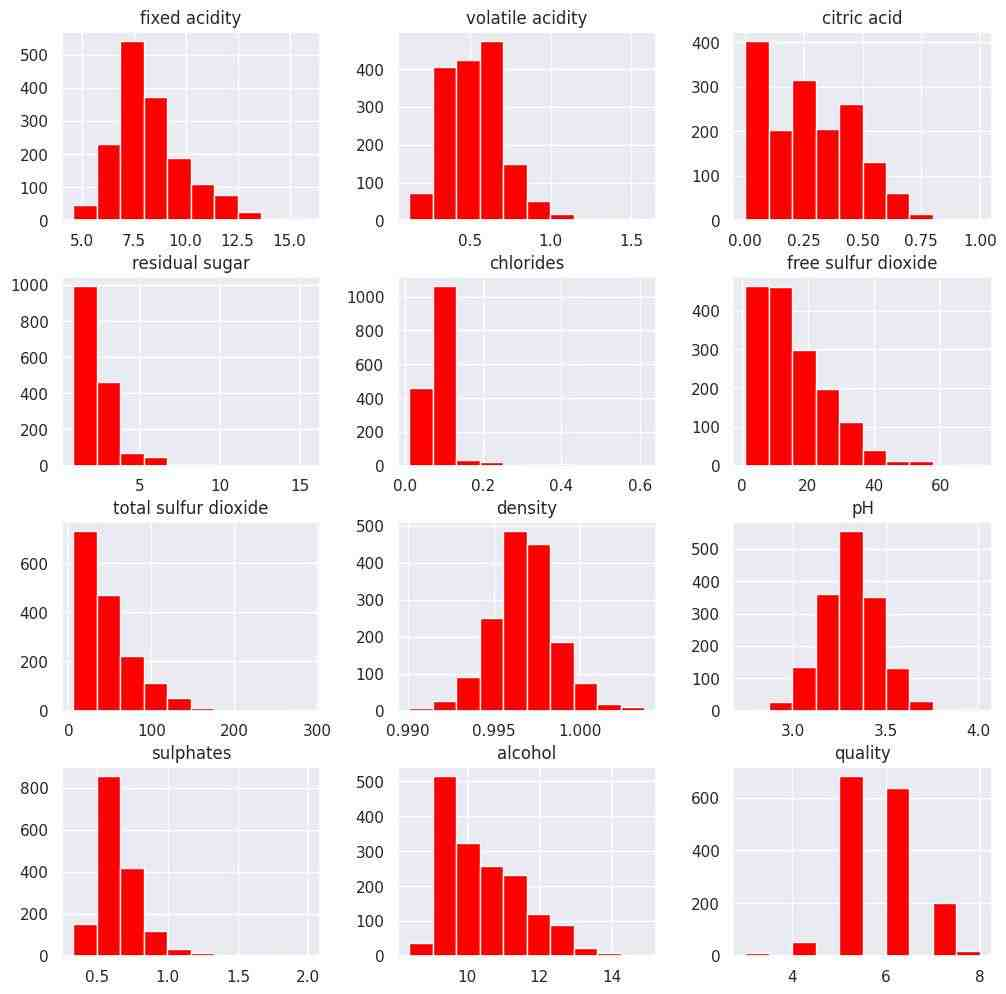
\includegraphics[width=\linewidth, height= 20cm]{Machine_learning/images/histogram_red.jpeg}
    \caption{Histogram plot of Red wine dataframe}
    \label{fig:enter-label}
\end{figure}

\newpage
\begin{lstlisting}[style=mypython]
sns.set()
white.hist(figsize=(12,12), color='red')
plt.show()
\end{lstlisting}
\begin{figure}[H]
    \centering
    \fbox{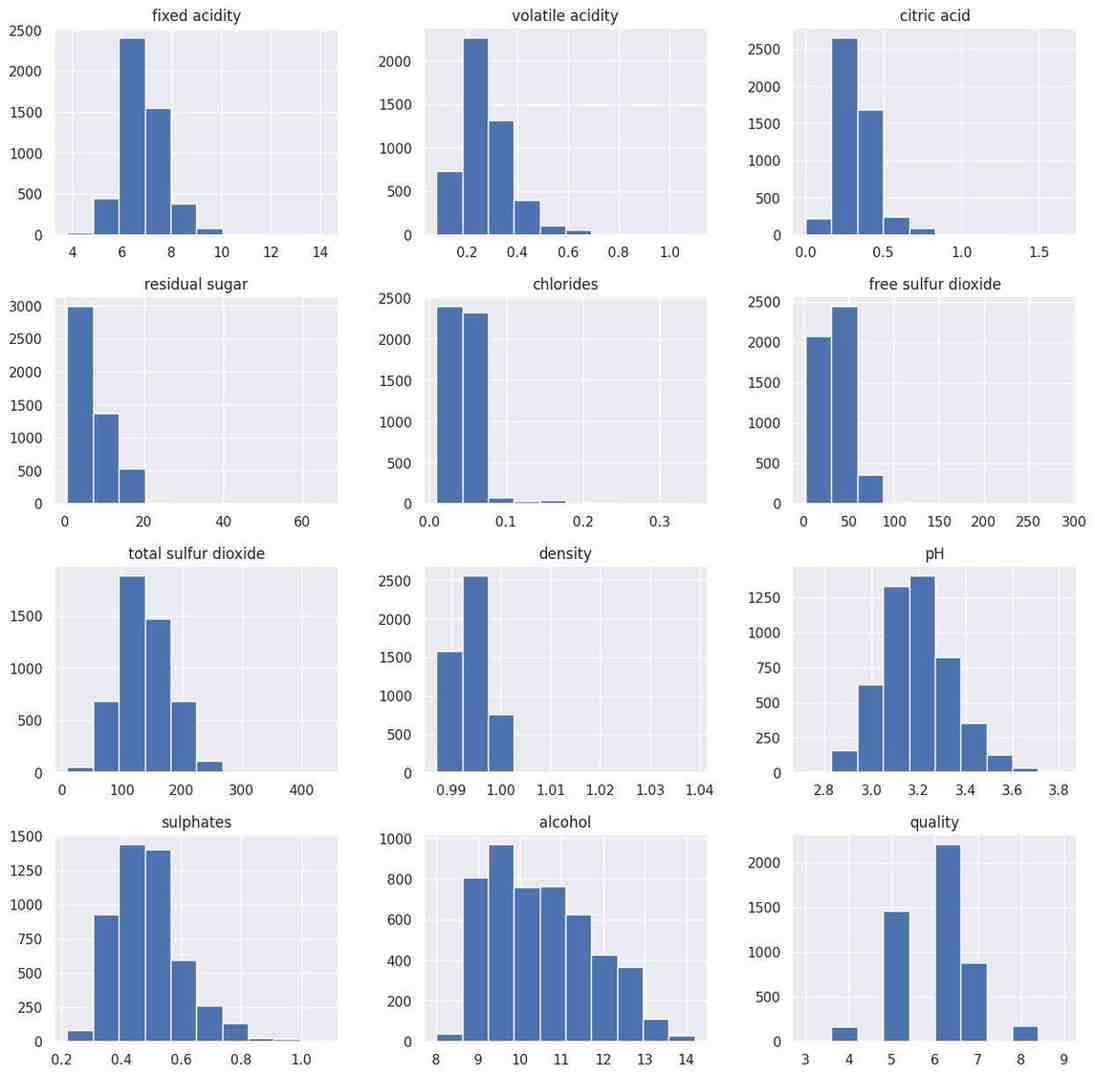
\includegraphics[width=\linewidth, height= 20cm]{Machine_learning/images/histogram_white.jpeg}}
    \caption{Histogram plot of White wine dataframe}
    \label{fig:enter-label}
\end{figure}

\newpage
\subsubsection{Box plot}
\begin{lstlisting}[style=mypython]
log_box = sns.boxplot(data=red_df, orient="h", palette="rainbow")
log_box.set_xscale("symlog")
log_box.axis(xmin=0, xmax=300)
\end{lstlisting}

\begin{figure}[H]
    \centering
    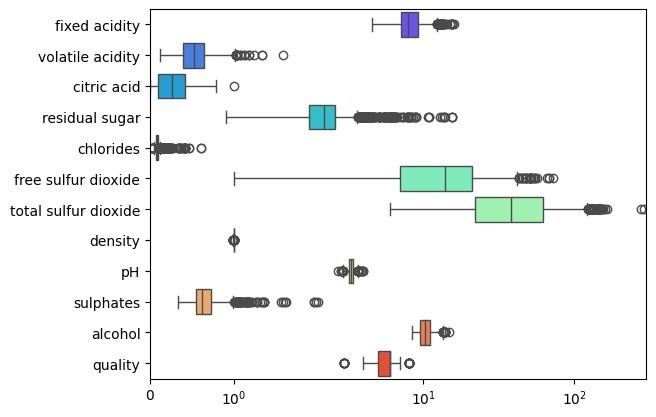
\includegraphics[width=0.8\linewidth]{Machine_learning/images/red_wine_box_plot.jpeg}
    \caption{log scale Box plot of Red wine dataset}
    %\label{fig:enter-label}
\end{figure}

\subsubsection{Violin plot}
\begin{lstlisting}[style=mypython]
sns.violinplot(x="quality", y="alcohol", data=red_df, hue="quality" ,palette="rainbow")
plt.show()
\end{lstlisting}

\begin{figure}[H]
    \centering
    \fbox{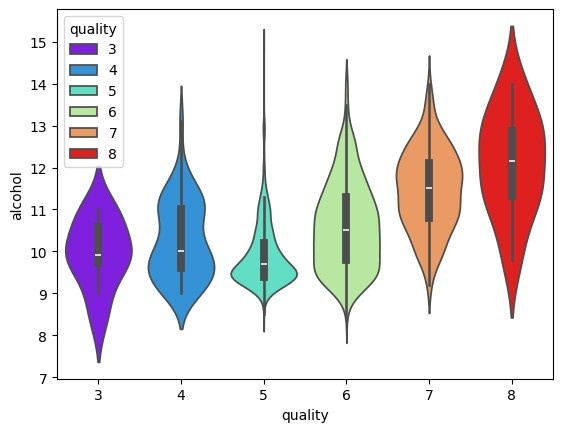
\includegraphics[width=10cm, height=8cm]{Machine_learning/images/red_quality_alcohol_violinplot.jpeg}}
    \caption{Violin plot between "quality" and "alcohol content" in red wine}
    %\label{fig:enter-label}
\end{figure}

\subsubsection{Heatmap}
\begin{lstlisting}[style=mypython]
red_correlation = red_df.corr(method='pearson')
fig=plt.gcf()
fig.set_size_inches(12,12)
sns.heatmap(red_correlation, annot=True,square=True, cmap="coolwarm")
\end{lstlisting}

\begin{figure}[H]
    \centering
    \fbox{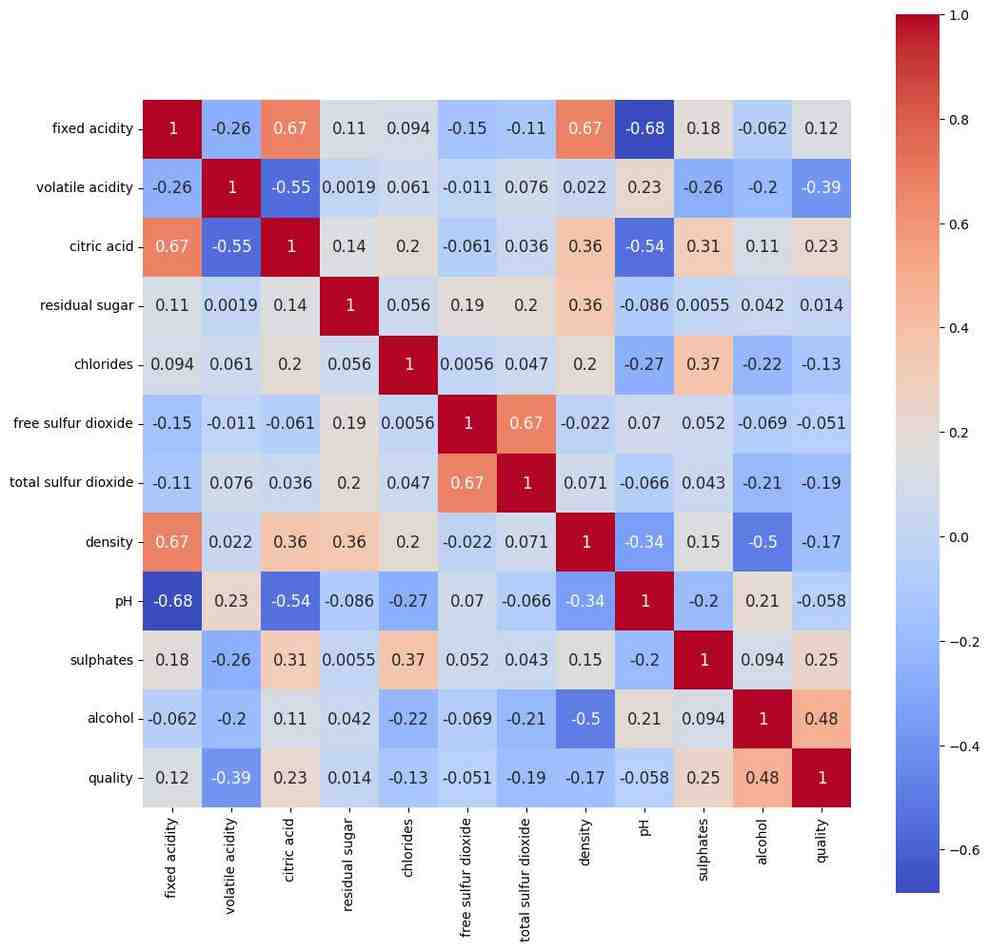
\includegraphics[width=\linewidth, height= 15cm]{Machine_learning/images/red_wine_heatmap.jpeg}}
    \caption{Correlation Heatmap of White wine dataset}
    %\label{fig:enter-label}
\end{figure}
\newpage
\begin{lstlisting}[style=mypython]
white_correlation = white_df.corr(method='pearson')
fig=plt.gcf()
fig.set_size_inches(12,12)
sns.heatmap(white_correlation, annot=True, square=True, cmap="coolwarm")
\end{lstlisting}

\begin{figure}[H]
    \centering
    \fbox{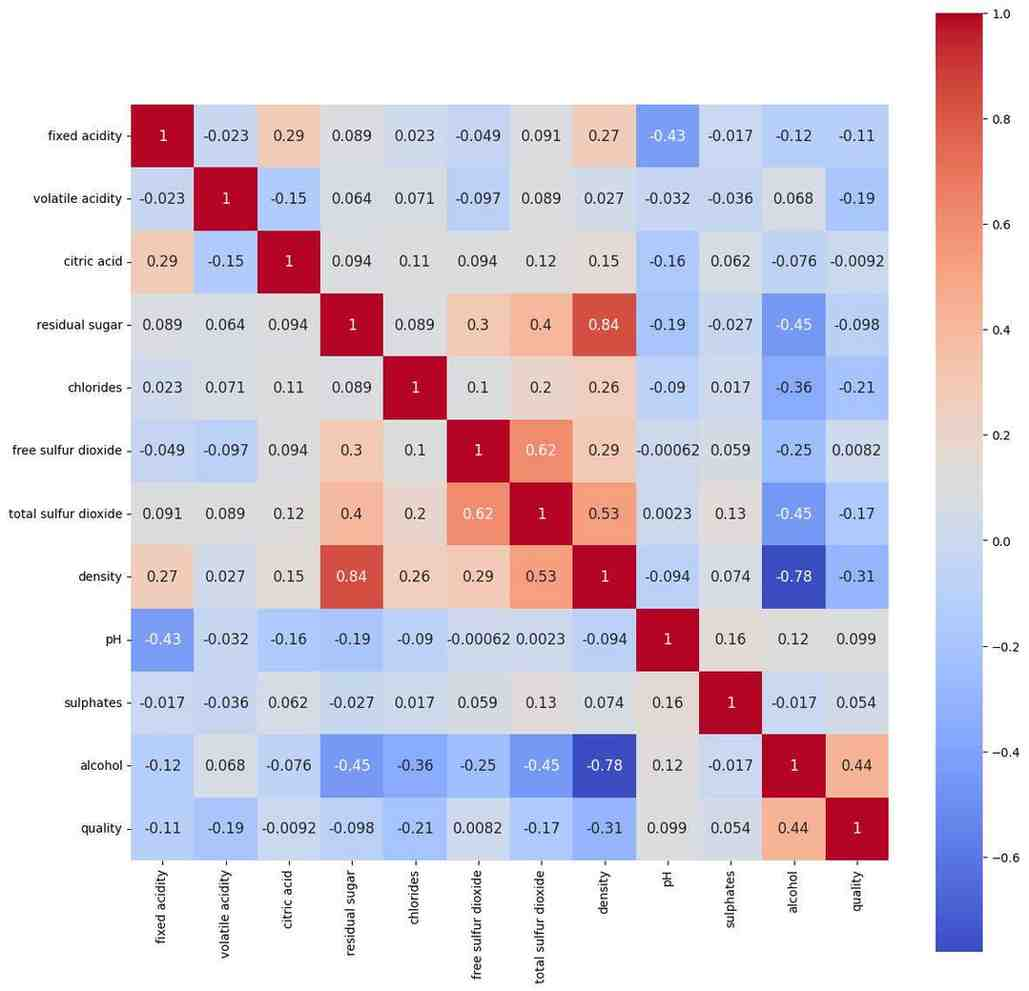
\includegraphics[width=17cm, height= 18cm]{Machine_learning/images/white_wine_heatmap.jpeg}}
    \caption{Correlation Heatmap of White wine dataset}
    \label{white_wine}
\end{figure}

\newpage
%Pair plot
\subsubsection{Pair plot}
\begin{lstlisting}[style=mypython]
sns.pairplot(red_df[['fixed acidity','volatile acidity','citric acid', 'pH']], corner=False) 
#corner=True hides the upper portion of the matrix
\end{lstlisting}
\begin{figure}[H]
    \centering
    \fbox{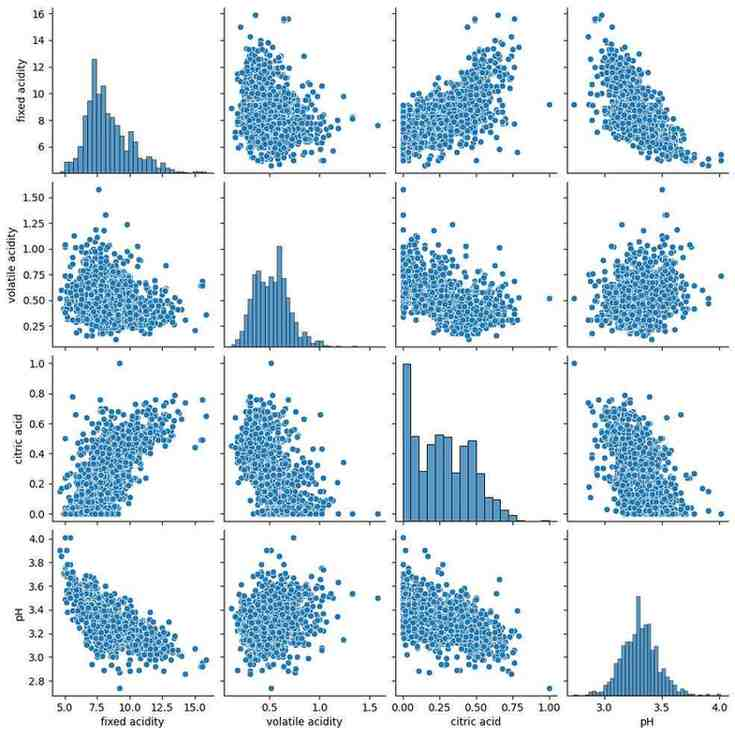
\includegraphics[width=\linewidth, height=19cm]{Machine_learning/images/pairplot_acid_pH.jpeg}}
    \caption{Pair scatterplot between "fixed acidity", "volatile acidity", "citric acid", "pH" of red wine dataset}
    %\label{fig:enter-label}
\end{figure}

\subsection{Statistics in pandas}
\subsubsection{Descriptive Statistics functions}
\begin{lstlisting}[style=mypython, caption={Statistics functions integrated with pandas}]
red_df.info() #Returns datatype and data range
red_df.head(10) # Returns first 10 row values
red_df.tail(10) #Returs last 10 row values
red_df.max(axis=0) #List out max value of all column variables
red_df["pH"].min() #Returns min value of "pH" column only
red_df.describe() #Returns count,mean,std,min,max & percentile
red_df.groupby(["quality"])[["alcohol"]].describe()
red_df.std(axis=0) #Returns standard deviation of all variables in column
\end{lstlisting}

\subsubsection{Confidence interval}
A confidence interval is a range of values derived from a sample data that is believed to contain the true value of an unknown population parameter with a specified probability. For example, if you calculate a $95\%$ confidence interval for a population mean, it means you are $95\%$ confident that the true mean lies within that interval based on the method and sample used. It can be mathematically formulated as:
\[
CI\;=\;Mean \pm z \times SE \quad where\;, \;SE = \frac{SD}{\sqrt{n}}
\]
\textbf{z} is the z-value, when calculating a confidence interval, is the value of the z (normal distribution) statistic for a certain confidence level. Common values of z for different confidence intervals are:\\
\[
\text{Confidence Level: } 90\%   \ (Z = 1.645), \quad 95\% \Rightarrow \ (Z = 1.96), \quad 99\% \Rightarrow\ (Z = 2.575)
\]
\textbf{SE} is the  Standard error of the mean. It indicates the uncertainty around the estimate of the mean.\\
\textbf{n} is the sample size

\subsection{Hypothesis tests}
When comparing two samples (or analytical methods) it's important to analyze if their means and/or variances are equal. In order to decide if the difference in their means and variances can be accounted to random variations, a statistical test can be used. These tests are also known as significance tests.
\begin{lstlisting}[style=mypython]
# Comparing only fixed acidity of red and white wine
fa_df = pd.concat([red_df["fixed acidity"],white_df["fixed acidity"]], ignore_index=True, axis=1)
fa_df.columns = ['red', 'white']
sns.boxplot(data = fa_df)
sns.violinplot(data = fa_df)
\end{lstlisting}

\begin{figure}[H]
    \centering
    \begin{minipage}[b]{0.48\linewidth}
        \centering
        \fbox{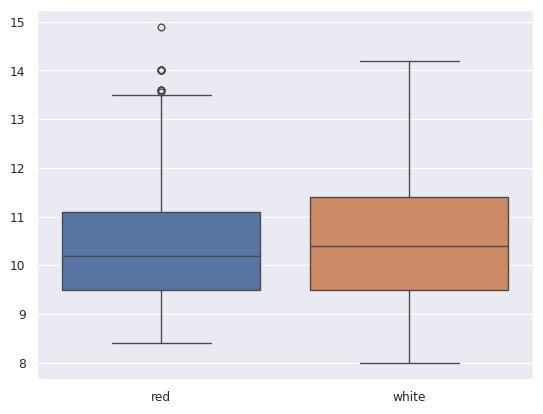
\includegraphics[width=\linewidth]{Machine_learning/images/hypothesis_alcohol_box.jpeg}}
        \caption*{(a) Alcohol content box plot}
    \end{minipage}
    \hfill
    \begin{minipage}[b]{0.48\linewidth}
        \centering
        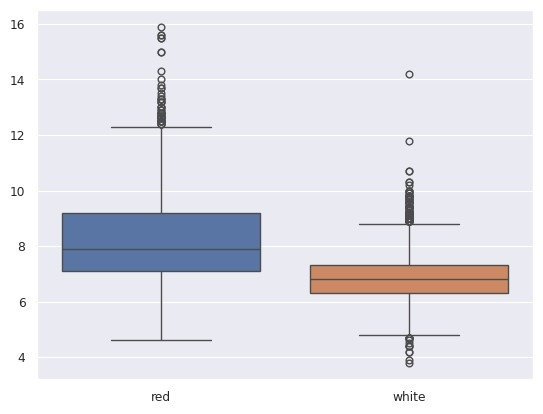
\includegraphics[width=\linewidth]{Machine_learning/images/hypothesis_test._box.jpeg}
        \caption*{(b) Fixed acidity box plot}
    \end{minipage}
    \caption{Hypothesis test plot between red and white wine}
    %\label{fig:side-by-side}
\end{figure}

\textbf{Conclusion from hypothesis test:} We notice that the distribution of alcohol content is very similar for red and white wines, while the distribution of fixed acidity is significantly different. Let's see if we can statistically demonstrate this observation.

\subsection{Student's t-test}
The Student's t-test is used to compare the mean of one or two normally distributed populations, preferably of equal size and variance by proposing an estimator of the likelihood of a Null Hypothesis. A distribution area related value called the "p-value" is then calculated. A very small p-value implies that Null Hypothesis is very unlikely. The usual criteria is to use a critical value of 0.05 for symmetrical distributions called the "level of significance"; if the calculated p-value is less than 0.05, then we conclude that the Null Hypothesis is very unlikely to be true.

\subsubsection{One-sample test}
In one-sample t-test we want to test the null hypothesis that the population mean $\bar x$ is equal to a specified value $\mu_0$. First we will determine the mean of the fixed acidity in our dataset.
\begin{lstlisting} [style=mypython]
fa_df.mean()    
Output:
red 	8.319637
white 	6.854788
\end{lstlisting}
Now that we know that the mean $(\bar x)$ for red wine is 8.31, we will compare it to the "true value" of 8.33 (that might have come from the certificate of analysis of a standard reference material for example).
\begin{lstlisting} [style=mypython]
test1=pg.ttest(fa_df['red'],8.33)
test1

Output:
| Test Type                | T-test        |
| T-statistic              | -0.237999     |
| Degrees of Freedom (dof) | 1598          |
| Alternative Hypothesis   | Two-sided     |
| p-value                  | 0.811912      |
| 95% Confidence Interval  | [8.23, 8.41]  |
| Cohens-d                 | 0.005952      |
| Bayes Factor (BF10)      | 0.029         |
| Statistical Power        | 0.056506      |

\end{lstlisting} 
As seen by the p-value (p-val= 0.81) the distribution mean could be 8.33. Let's perform the test again using a "true" white wine mean of 6.85.

\begin{lstlisting} [style=mypython]
test2=pg.ttest(fa_df['red'],6.85)
test2
Output:
| Test Type                | T-test                      |
| T-statistic              | 33.752939                   |
| Degrees of Freedom (dof) | 1598                        |
| Alternative Hypothesis   | Two-sided                   |
| p-value                  | 5.398298e-189               |
| 95% Confidence Interval  | [8.23, 8.41]                |
| Cohens-d                 | 0.844087                    |
| Bayes Factor (BF10)      | 8.726e184                  |
| Statistical Power        | NaN                         |

\end{lstlisting}

In this case, the p-value is $5.39 e^{-189}$. This means it is not probable that 6.85 is the $(\mu_0)$ of the fixed acidity content for red wine.

\subsubsection{Two-sample test}
We can directly compare the fixed acidity values for both kinds of wine by using a two independent sample t-test (since the wines we are analyzing are independent). The independence of the samples is indicated with the parameter paired=False.

The correction parameter is used when both populations have different sample sizes, by setting it to "auto", it will automatically apply a correction when the sample sizes are unequal. This correction uses an equation called Welch-Satterthwaite's equation, that implies making complicated calculations involving the standard deviations.
\begin{lstlisting}[style=mypython]
fa_df["white"].dropna()
print(fa_df.mean())
test3=pg.ttest(fa_df['red'],fa_df['white'], paired=False,correction='auto')
test3
Output:
red      8.319637
white    6.854788

| T           | 32.422711     |
| dof         | 1848.947934   |
| alternative | two-sided     |
| p-val       | 5.668161e-183 |
| CI95%       | [1.38, 1.55]  |
| cohen-d     | 1.293371      |
| BF10        | 4.834e+209    |
| power       | 1.0           |
\end{lstlisting}

\begin{lstlisting} [style=mypython]
# Two sample t-test for alcohol content
print(al_df.mean())
test4=pg.ttest(al_df['red'],al_df['white'], paired=False,correction='auto')
test4
Output:
red      10.422983
white    10.514267

| T           | -2.859029       |
| dof         | 3100.474621     |
| alternative | two-sided       |
| p-val       | 0.004278        |
| CI95%       | [-0.15, -0.03]  |
| cohen-d     | 0.076571        |
| BF10        | 1.903           |
| power       | 0.757462        |
\end{lstlisting}


As the p-value is less than 0.05, we can say the difference in alcohol content is statistically significant. This points to a strong evidence against the null hypothesis, meaning we can safely say that both populations are different.

Upon inspection, we can see that the value for the degrees of freedom (DOF) is a decimal number. Given that the degrees of freedom should be (N-1), N being the sample size, one would expect N to be a whole number. As the sample size for red wine is smaller than the one for white wine (1599 vs 4898), the pingouin library estimated the DOF using the Welch–Satterthwaite equation. That's also why the DOF differs for "alcohol" and "fixed acidity", in both the sample size is the same but they have different standard deviations. If we use the parameter correction="auto" pengouin will use the W.S equation even if the sample size is the same for each column.

In case we needed to compare the results of a certain treatment on a material system or population (where the two groups of measure would be dependent), the correct way to perform a two sample t-test would be to indicate that the samples are dependent; this is usually called a paired t-test.


\subsection{Equality of Variances (Homoscedasticity)}
A common assumption for many tests is that the variance for the different sets must be the same. So it's always handy to have a tool that can check this assumption before processing. You must have heard of the F-test. It's the simplest test for this job, however there are many more robust and powerful tests, and Pingouin doesn't offer an F-test function in his repertory. However another common test is Levene's test, which is more robust regarding lack of normality and more suitable on many situations (W statistic that follows an F distribution). Pingouin also offers another common test called Bartlett's test.

\begin{lstlisting} [style=mypython]
print('SD of "alcohol content": \n',al_df.std())
Output:
SD of "alcohol content": 
 red      1.065668
white    1.230621
\end{lstlisting}

\begin{lstlisting} [style=mypython]
test5=pg.homoscedasticity(data=[red_df["alcohol"].to_numpy(),white_df["alcohol"].to_numpy()], alpha=0.05)
test5
Output:
levene test
| W          | 72.784614    |
| pval       | 1.780219e-17 |
| equalvar   | False        |
\end{lstlisting}


\subsection{ANOVA}
ANOVA (Analysis of Variance) is a statistical test used to determine whether the means of multiple groups are significantly different. It requires a categorical independent variable (E.g., wine quality) and a continuous dependent variable (E.g., residual sugar or alcohol content). ANOVA compares the within-group variance to the between-group variance and computes an F-statistic along with a p-value. A low p-value suggests that at least one group mean differs significantly. For example, using the wine dataset, we can compare the mean residual sugar across different quality levels (3 to 10). Pingouin provides a simple method to perform ANOVA directly on pandas DataFrames.
\begin{lstlisting} [style=mypython]
red_df.anova(dv="residual sugar", between="quality")
Output:
| Source     | quality   |
| ddof1      | 5         |
| ddof2      | 1593      |
| F          | 1.053374  |
| p-unc      | 0.384619  |
| np2        | 0.003295  |
\end{lstlisting}
Here \textbf{dv} means dependent variable, \textbf{between }='quality' means that 'quality' is our independent (categorical) variable.
We could safely conclude from this analysis, given the high p-value (>0.05, here stated as "p-unc"), that the residual sugar will be the same regardless of the quality of the wine (or at least the mean of all the wines that were analyzed).

Let's analyze another variable, like the alcohol content, and let's see if we arrive to a different conclusion:
\begin{lstlisting} [style=mypython]
red_df.anova(dv="alcohol", between="quality")
Output:
| Source     | quality       |
| ddof1      | 5             |
| ddof2      | 1593          |
| F          | 115.854797    |
| p-unc      | 1.209895e-104 |
| np2        | 0.266667      |
\end{lstlisting}
A we can see, the p-value is too low, so we can say for sure that at least two values of alcohol content of wines of different qualities are indeed different.


\subsection{Variable Reduction}
A very useful way to visualize data with multiple variables are variable reduction techniques. Which reduce the multiple dimensions of the problem to just two or three, in order to make a plot that allows us to visualize the overall distribution of the variables.
We will concatenate the datasets of red and white wine for the Purposes of visualization.

\subsubsection{PCA (Principal Components Analysis)}
The PCA algorithm defines a new set of coordinates (components) from a large dataset with multiple variables, and transforms the values into the new coordinates. These coordinates are defined in order to maximize the variance by some scalar projection. The components are arranged according to their original variance, that's why this technique is useful for reducing the dimensions of a dataset.

After loading the dataset, we import the Standard Scaler from $\texttt{sklearn.preprocessing}$ and PCA function from $\texttt{sklearn.decomposition}$. Scaling the data is important as not every variable has the same range. So, we create the PCA object and define the number of components. Using $\texttt{StandardScaler()}$ and $\texttt{fit\_transform()}$, we can fit the new variables (components) and transform their values into the new variables. $\texttt{StandardScaler()}$ does scaling the data. The $\texttt{fit\_transform()}$ module fits these new values to the data, and stores them, replacing the old values.


This is the most fastest variable reduction technique as it only uses basic algebra equation for finding Principle Components 1 \& 2 and it will use them to plot a graph. But it can be use only for linear data. Since for non-linear data, the principle components will overlap with each other and the result is not consistent.

\begin{lstlisting}[style=mypython]
from sklearn.preprocessing import StandardScaler
from sklearn.decomposition import PCA

data_pca = df_wine.copy()
data_pca = data_pca.drop(labels = ['quality', 'hue'],axis = 1)
data_pca = StandardScaler().fit_transform(data_pca)
#Apply PCA on the transformed (scaled and centered) data:
pca = PCA(n_components=3)
pca_results = pca.fit_transform(data_pca)
pca_results

Output:
array([[-3.20599617,  0.41652332, -2.72223659],       [-3.03905081,  1.10746213, -2.04695235],
       [-3.07189347,  0.87896444, -1.74257961],       ...,
       [ 0.5711325 , -0.72266165,  0.09146896],       [ 0.09005243, -3.54577991,  0.14119458],
       [ 0.51257566, -2.89104008,  0.73941657]])
\end{lstlisting}

\begin{lstlisting}[style=mypython]
pca_dataset = pd.DataFrame(data = pca_results, columns = ['component1', 'component2','component3'] )
pca_dataset['hue']=df_wine['hue']
plt.figure()
plt.figure(figsize=(6,6))
plt.xlabel('Component 1')
plt.ylabel('Component 2')
plt.title('2 Component PCA')
sns.scatterplot(x = pca_dataset['component1'], y = pca_dataset['component2'], hue=pca_dataset['hue'],alpha=1,palette=["red", "blue"])
\end{lstlisting}

\begin{figure}[H]
    \centering
    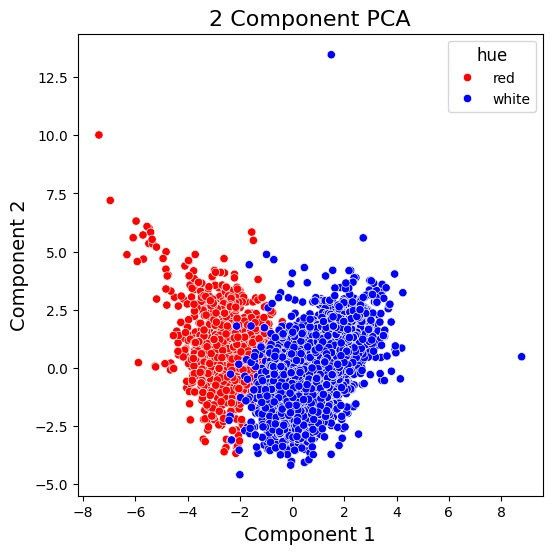
\includegraphics[width=\linewidth]{Machine_learning/images/PCA.jpeg}
    \caption{2-dimensional PCA plot}
    %\label{fig:enter-label}
\end{figure}

\subsubsection{t-SNE (t-distributed Stochastic Neighbor Embedding)}
t-SNE is an algorithm that determines the similarity between pairs of points in a high dimensional space and replicates this similarity in a low dimensional space based on the probability distribution of the distances.

We can make this dimension reduction with the scikit learn module and then plot it with seaborn. First, we make a copy of the dataset, then, we drop the columns for quality and wine in this copy, as we won't be using them to make the t-SNE, but we will take the wine column into account for the plot, for the purpose of visualization.

To make the dimension reduction we have to create a t-SNE object and then use the $\texttt{tsne.fit\_transform()}$ function on it with our dataset copy.

\begin{lstlisting} [style=mypython]
from sklearn.manifold import TSNE
data_tsne = df_wine.copy()
data_tsne = data_tsne.drop(labels = ['quality', 'hue'],axis = 1)
data_tsne = StandardScaler().fit_transform(data_tsne)
tsne = TSNE(n_components=2, verbose=1, perplexity=40, n_iter=300)
tsne_results = tsne.fit_transform(data_tsne)    
\end{lstlisting}

\begin{lstlisting} [style=mypython]
tsne_dataset = pd.DataFrame(data = tsne_results, columns = ['component1', 'component2'] )
tsne_dataset['hue']=df_wine['hue']
plt.figure()
plt.figure(figsize=(10,10))
plt.xlabel('Component 1')
plt.ylabel('Component 2')
plt.title('2 Component TSNE')
sns.scatterplot(x = tsne_dataset['component1'], y = tsne_dataset['component2'], hue=tsne_dataset['hue'],alpha=1, palette=["red", "blue"])
plt.legend()    
\end{lstlisting}


\begin{figure}[H]
    \centering
    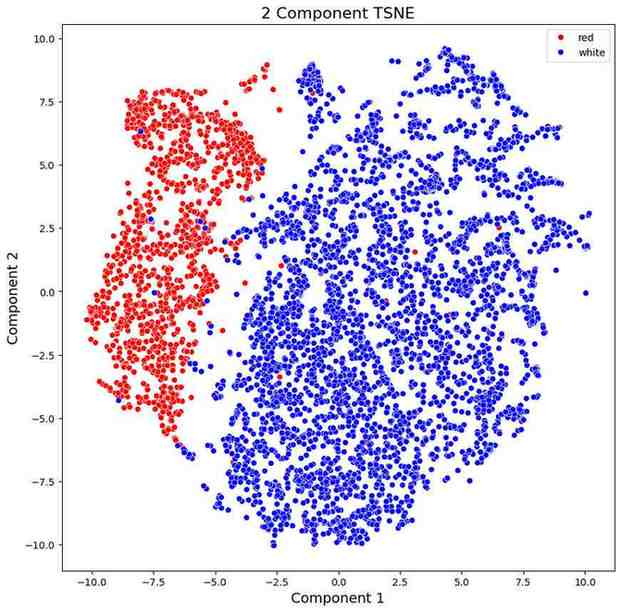
\includegraphics[width=0.9\linewidth]{Machine_learning/images/tsne.jpeg}
    \caption{2-dimensional t-SNE plot}
    %\label{fig:enter-label}
\end{figure}


\subsubsection{UMAP (Uniform Manifold Approximation and Projection)}
UMAP is a new technique published in 2018 for dimension reduction. This is an alternative to t-SNE for visualization, that preserves more of the global structure with better run time performance. The data is modeled by a manifold with a fuzzy topological structure. The small representation (or embedding) is found by searching for a low dimensional projection of the data that has the closest possible equivalent fuzzy topological structure.

\begin{lstlisting} [style=mypython]
import umap
data_umap = df_wine.copy()
data_umap = data_umap.drop(labels = ['quality', 'hue'],axis = 1)
scaled_data_umap = StandardScaler().fit_transform(data_umap) #We convert each feature into z-scores (number of standard deviations from the mean) for comparability.
umap = umap.UMAP()
umap_results = umap.fit_transform(scaled_data_umap)
umap_results

Output:

array([[ 2.0228717 , -0.65424883],
       [ 1.4935756 , -0.4979152 ],
       [ 1.3704098 , -0.3243352 ],
       ...,
       [11.418766  ,  7.4003463 ],
       [ 8.92388   , 12.713315  ],
       [ 8.568939  , 11.276885  ]], dtype=float32)
\end{lstlisting}

\begin{lstlisting} [style=mypython]
umap_dataset = pd.DataFrame(data = umap_results, columns = ['component1', 'component2'] )
umap_dataset['hue']=df_wine['hue']
plt.figure()
plt.figure(figsize=(10,10))
plt.xlabel('Component 1')
plt.ylabel('Component 2')
plt.title('2 Component UMAP')
sns.scatterplot(x = umap_dataset['component1'], y = umap_dataset['component2'], hue = umap_dataset['hue'],alpha=1,palette=["red", "blue"])
\end{lstlisting}

\begin{figure}[H]
    \centering
    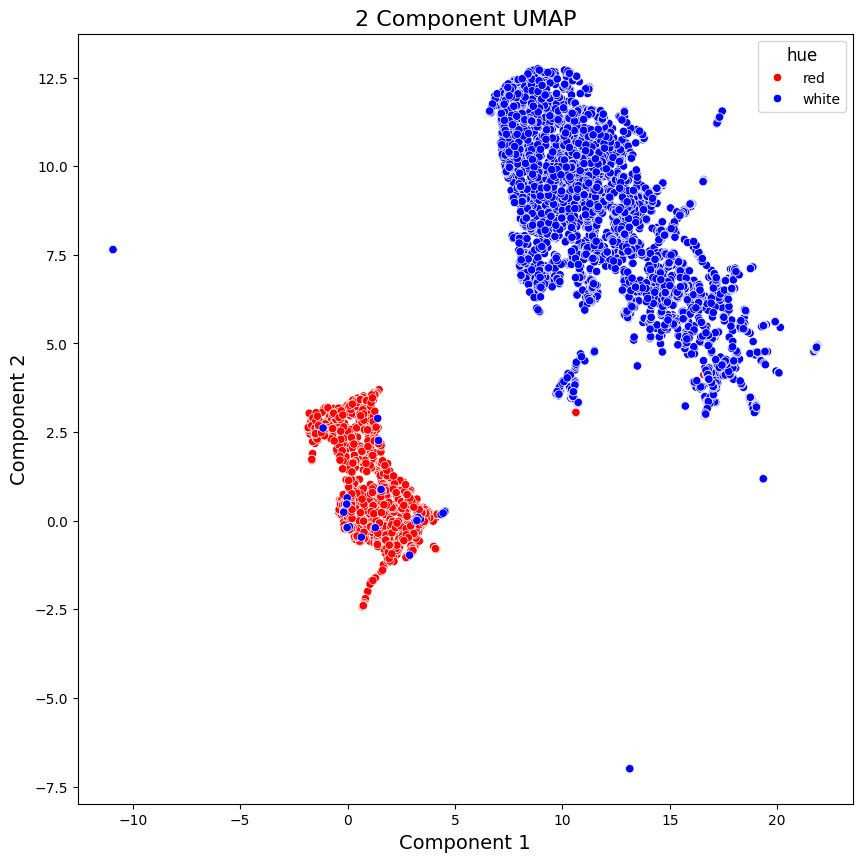
\includegraphics[width=0.7\linewidth]{Machine_learning/images/umap.jpeg}
    \caption{2-dimensional UMAP plot}
    %\label{fig:enter-label}
\end{figure}


\subsection{Classification}
\subsubsection{Logistic regression}
Logistic regression is a basic classification method. It is based on the logistic function which is a general form of the sigmoid function. It is an S-shaped curve that can take any real-valued number in the x-axis and values between 0 and 1 on the y axis. It can be used to classify between two classes (0 and 1). The y value expresses the probability that class 1 occurs.
\begin{lstlisting} [style=mypython]
df_LR = red_df.loc[(red_df['quality'] == 3 ) | (red_df['quality'] == 8 ), ['alcohol','quality']]

df_LR.loc[df_LR.quality == 3, 'quality'] = 0
df_LR.loc[df_LR.quality == 8, 'quality'] = 1

df_LR.plot.scatter(x = 'alcohol', y = 'quality')   
\end{lstlisting}



\begin{lstlisting} [style=mypython]
sns.regplot(x="alcohol", y="quality",data=df_LR, logistic=True, scatter_kws={'color': 'blue'}, line_kws={'color': 'green'})
plt.show()    
\end{lstlisting}

\begin{lstlisting} [style=mypython]
from sklearn.linear_model import LogisticRegression
X = df_LR[['alcohol']]
y = df_LR.quality
model = LogisticRegression(C = 1e9)
model.fit(X, y)    
\end{lstlisting}


\begin{lstlisting} [style=mypython]
from scipy.special import expit
x_test = np.linspace(8.5,14.0,100)
# predict dummy y_test data based on the logistic model
y_test = x_test * model.coef_ + model.intercept_
sigmoid = expit(y_test)
plt.scatter(X,y)
# ravel to convert the 2-d array to a flat array
plt.plot(x_test,sigmoid.ravel(),c="green", label = "logistic fit")
plt.legend(loc="lower right")    
\end{lstlisting}

\begin{figure}[H]
    \centering
    \begin{minipage}[b]{0.48\linewidth}
        \centering
        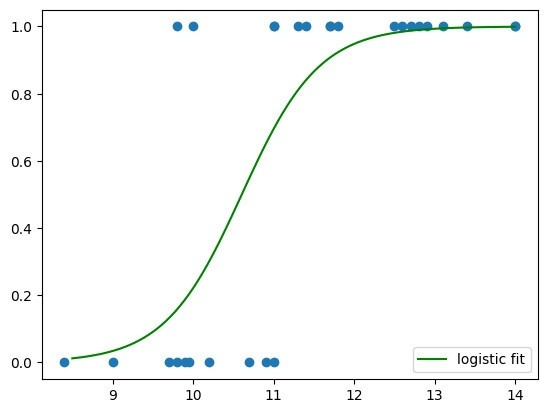
\includegraphics[width=\linewidth]{Machine_learning/images/log_reg.jpeg}
        \caption*{(a) Logistic Regression plot}
    \end{minipage}
    \hfill
    \begin{minipage}[b]{0.48\linewidth}
        \centering
        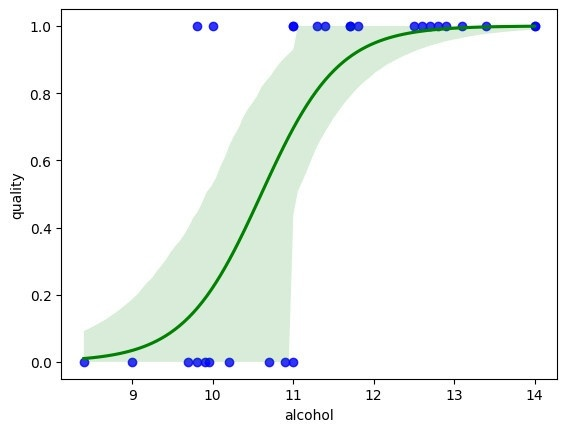
\includegraphics[width=\linewidth]{Machine_learning/images/log_reg2.jpeg}
        \caption*{(b)  Logistic Regression plot}
    \end{minipage}
    \caption{Hypothesis test plot}
    %\label{fig:side-by-side}
\end{figure}


\subsubsection{Data Splitting and Standardization}
\label{Data_split}
In general, the data is split into two groups before generating a model. These groups are called training and testing sets. The training set is used for developing models and select the parameters that are adequate for the data. The test set is used to assess the performance of the model with previously unseen data. The most common way is to divide the data is random splitting.

We will split the dataset using the function $\texttt{train\_test\_split()}$ from scikit learn. The training set is $67\%$ of the data and the test set is $33\%$ (We have deliberately specified it that way in the parameters). The $\texttt{random\_state}$ parameter controls the shuffling applied to the data before applying the split.

Standardization is a method to transform variables that differ in mean and deviation into comparable values. This process consists of subtracting the means from each feature and then dividing by the feature standard deviation. Many machine learning algorithms assume that all features are centered around zero and have approximately the same variance, then standardization is needed.

In this case, we will use the function $\texttt{StandardScaler()}$. It will first fit the data to determine the mean and standard deviation and then transform it into a standardized form. 

\begin{lstlisting} [style=mypython]
#Data splitting
from sklearn.model_selection import train_test_split
X = df_wine.drop(['quality', 'hue'], axis=1)
y = df_wine['hue']
X_train, X_test, y_train, y_test = train_test_split(X, y, test_size=0.33, random_state=42)    
\end{lstlisting}


\begin{lstlisting} [style=mypython]
# Data Standardization
from sklearn import preprocessing
scaler = preprocessing.StandardScaler()
scaler.fit(X_train)
X_train = scaler.transform(X_train)
X_test = scaler.transform(X_test)    
\end{lstlisting}

\begin{lstlisting} [style=mypython]
from sklearn.linear_model import LogisticRegression
from sklearn.metrics import classification_report, accuracy_score, confusion_matrix

lr = LogisticRegression(random_state=0) #random_state parameter is provided to control the random number generator used whenever randomization is part of a Scikit-learn algorithm.
lr.fit(X_train, y_train)   
\end{lstlisting}

\subsubsection{Multiple Logistic Regression}
In this case, we will use all the features with logistic regression to classify white and red wine.
\begin{lstlisting} [style=mypython]
from sklearn.linear_model import LogisticRegression
from sklearn.metrics import classification_report, accuracy_score, confusion_matrix
lr = LogisticRegression(random_state=0) #random_state parameter is provided to control the random number generator used whenever randomization is part of a Scikit-learn algorithm.
lr.fit(X_train, y_train)   
\end{lstlisting}

\begin{lstlisting} [style=mypython]
y_pred = lr.predict(X_test)
print("Accuracy score: " + str(accuracy_score(y_test, y_pred)))
print("\nConfusion matrix: \n" + str(confusion_matrix(y_test, y_pred)))
print("\nClassification report: \n" + str(classification_report(y_test, y_pred)))

Output: 

Accuracy score: 0.9888111888111888

Confusion matrix: 
[[ 544   13]
 [  11 1577]]

Classification report: 
              precision    recall  f1-score   support

           0       0.98      0.98      0.98       557
           1       0.99      0.99      0.99      1588

    accuracy                           0.99      2145
   macro avg       0.99      0.98      0.99      2145
weighted avg       0.99      0.99      0.99      2145

\end{lstlisting}

% \begin{lstlisting} 

% \end{lstlisting}
% \begin{lstlisting} [style=mypython]

% \end{lstlisting}


\subsection{Performance Metrics for Classification}
The metrics are the values that guide the decision in machine learning. For example, choosing what model performs better or what parameters improve a model by measuring and comparing among different cases. In this section, we are going to analyze some of the most used metrics for the classification task.

Accuracy in this context of classification problems is the number of correct predictions over the total amount of predictions. This metric is useful when the classes to classify are approximately balanced. It is expected that the accuracy is better on the training set than on the test set.

\begin{lstlisting} [style=mypython]
train_accuracy = lr.score(X_train, y_train)
test_accuracy = lr.score(X_test, y_test)
print('One-vs-rest', '-'*35,
'Accuracy in Train Group   : {:.3f}'.format(train_accuracy),
'Accuracy in Test  Group   : {:.3f}'.format(test_accuracy), sep='\n') 

Output:

One-vs-rest
-----------------------------------
Accuracy in Train Group   : 0.995
Accuracy in Test  Group   : 0.989
\end{lstlisting}

\begin{figure}[H]
    \centering
    \begin{minipage}[b]{0.48\linewidth}
        \centering
        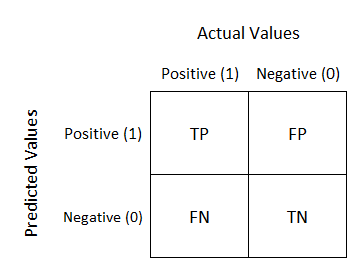
\includegraphics[width=\linewidth]{Machine_learning/images/confusion1.png}
        \caption*{(a) Confusion matrix structure}
    \end{minipage}
    \hfill
    \begin{minipage}[b]{0.48\linewidth}
        \centering
        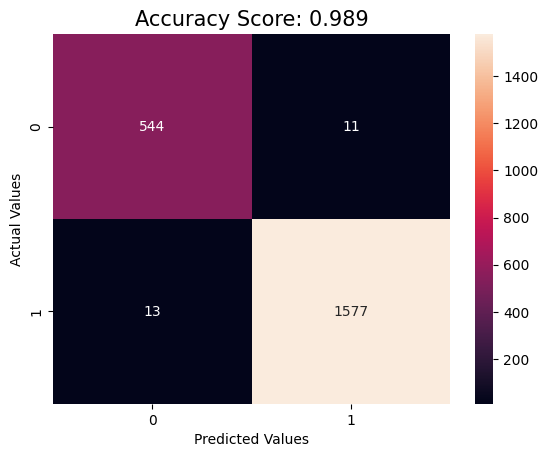
\includegraphics[width=\linewidth]{Machine_learning/images/confusion2.png}
        \caption*{(b) Confusion matrix of training dataset}
    \end{minipage}
    %\caption{Hypothesis test plot}
    %\label{fig:side-by-side}
\end{figure}

\subsubsection{Confusion Matrix}
 The Confusion Matrix is used for visualized the performance in a classification problem of two or more types of classes. For a binary case as ours, we compared the “Actual” vs “Predicted” values and obtain 4 cases:
\textbf{TP} - True Positive
\textbf{TN }- True Negative
\textbf{FP }- False Positive
\textbf{FN }- False Negative

\begin{lstlisting} [style=mypython]
from sklearn.metrics import confusion_matrix as cm
predictions = lr.predict(X_test)
score = round(accuracy_score(y_test, predictions), 3)
cm1 = cm(predictions, y_test)
sns.heatmap(cm1, annot=True, fmt=".0f")
plt.xlabel('Predicted Values')
plt.ylabel('Actual Values')
plt.title('Accuracy Score: {0}'.format(score), size = 15)
plt.show()
\end{lstlisting}

\subsubsection{Precision score}
The precision is a metric that informs how many positive-predicted instances were actually positive.
\[
Precision= \frac{TP}{TP+FP}
\]
\begin{lstlisting} [style=mypython]
from sklearn.metrics import precision_score
print("precision score: ",  precision_score(y_test, predictions, average='micro'))

Output:
precision score:  0.9888111888111888
\end{lstlisting}

\subsubsection{Recall score}
The recall is a metric that informs how many instances were identified correctly of all the positive classes.
\[
Recall= \frac{TP}{TP+FN}
\]
\begin{lstlisting} [style=mypython]
from sklearn.metrics import recall_score
print("recall score: ",  recall_score(y_test, predictions, average='micro'))

Output:
recall score:  0.9888111888111888
\end{lstlisting}

\subsubsection{F1 score}
The $F1-Score$ is a metric that shows the harmonic mean of precision and recall.
\[
F_1 \;Score=\frac{2\times Recall\times Precision}{Recall+Precision}
\]

\begin{lstlisting} [style=mypython]
from sklearn.metrics import f1_score
precision_s = precision_score(y_test, predictions,average='micro')
recall_s    = recall_score(y_test, predictions, average='micro')
print("F1_score     : ",  2*((precision_s*recall_s)/(precision_s + recall_s)))

Output:
F1_score:  0.9888111888111888
\end{lstlisting}


\subsection{Decision tree}
A decision tree is a non-linear technique that splits the dataset into subsets based on a feature value. This step is repeated recursively on each new subset until some criteria are reached. For example, every point in the subset has the same value of the target variable, or a maximum depth is attained. Choosing the feature and value to split is based on reducing the target entropy by dividing into pure subsets. An interesting feature of the decision trees is that we can generate an scheme that shows us how the decisions that were made.
\begin{lstlisting} [style=mypython]
from sklearn import tree
from sklearn.tree import DecisionTreeClassifier
dt = DecisionTreeClassifier(criterion = 'entropy', max_depth = 3, random_state = 1)
dt.fit(X_train, y_train)
y_pred = dt.predict(X_test)
print("Accuracy score: " + str(accuracy_score(y_test, y_pred)))
print("\nConfusion matrix: \n" + str(confusion_matrix(y_test, y_pred)))
print("\nClassification report: \n" + str(classification_report(y_test, y_pred)))

Output:
Accuracy score: 0.9724941724941725

Confusion matrix: 
[[ 522   35]
 [  24 1564]]

Classification report: 
              precision    recall  f1-score   support

           0       0.96      0.94      0.95       557
           1       0.98      0.98      0.98      1588

    accuracy                           0.97      2145
   macro avg       0.97      0.96      0.96      2145
weighted avg       0.97      0.97      0.97      2145
\end{lstlisting}

\begin{lstlisting} [style=mypython]
fig = plt.subplots(figsize=(20, 8))
tree.plot_tree(dt, fontsize=12)
\end{lstlisting}
\begin{figure}[H]
    \centering
    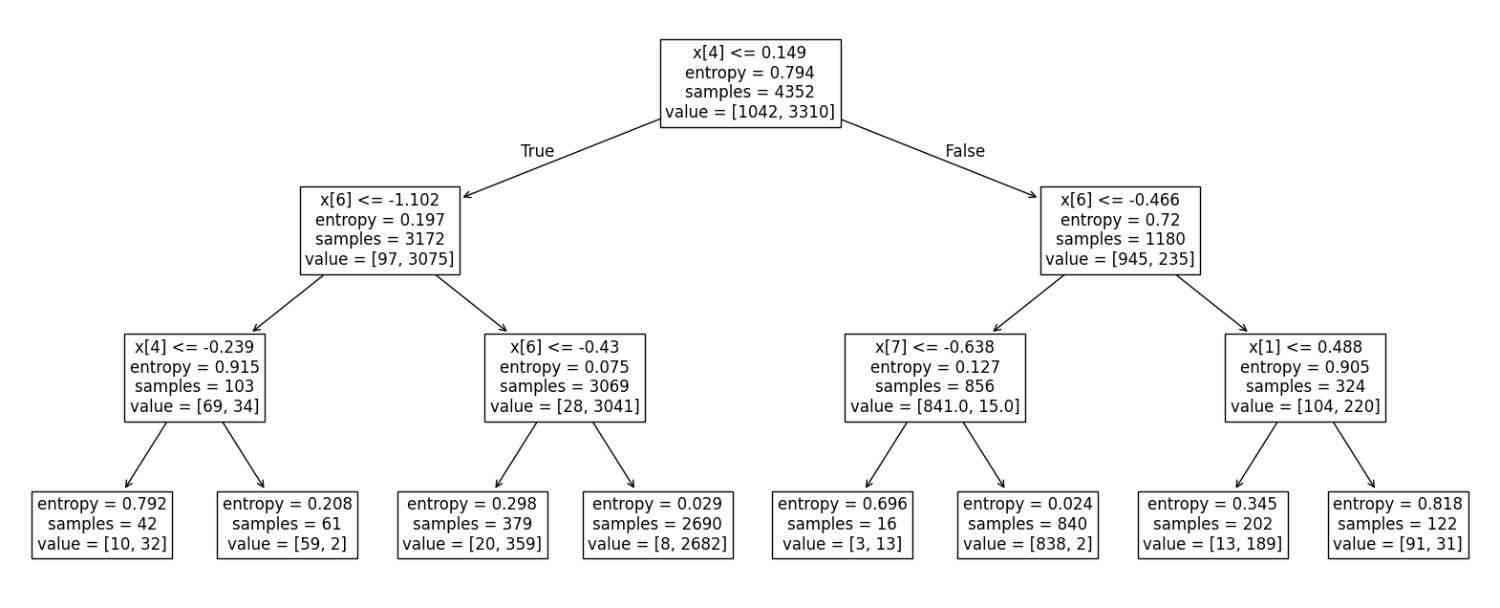
\includegraphics[width=\linewidth]{Machine_learning/images/decision_tree.jpeg}
    \caption{Decision tree plot for three generations.}
    %\label{fig:enter-label}
\end{figure}

\subsection{Regression}
\subsubsection{Correlation}
To fit the data with a linear model regression, it is a good practice to employ variables presenting a high correlation with the target. One way to do this is by calculating correlation coefficients and another way is through visual methods.
We will predict the density for red wines, so we import the data and then inspect the dataset.
From white wine correlation heatmap in \cref{white_wine}. We can look the variables which are related to density of wine.

\subsubsection{Linear Regression}
\label{linear_reg}
After the correlation analysis we will perform a linear regression using alcohol as the predictor variable $(x_i)$ and density as the target $(y_i)$, according to the model:
\[
(y_i)=\beta_1 x_i+\beta_0
\]

We will split the data into training and test sets, which is commonly done in machine learning methods for validation of the model created. It is the same method we used in \cref{Data_split}

\begin{lstlisting} [style=mypython]
from sklearn.linear_model import LinearRegression
linear_regression = LinearRegression()
linear_regression.fit(X = X_train, y = y_train)
# Let's print the parameters of the linear regression.
print('Beta1 = ' + str(linear_regression.coef_) + ', Beta0 = ' + str(linear_regression.intercept_))

Output:
Beta1 = [-0.00190561], Beta0 = 1.01408716780891
\end{lstlisting}


We can quantify how good the adjustment was by using the $R^2$ parameter. The adjustments usually are better on the training sets than the test sets, but in this case, we will find that the training set has some outliers that make this adjustment for the training set worse.
\[
R^2 = 1 - \frac{\sum (y_i - \hat{y}_i)^2}{\sum (y_i - \bar{y})^2}
\]


\begin{lstlisting} [style=mypython]
from sklearn.metrics import r2_score
y_pred_test = linear_regression.predict(X_test)
y_pred_train = linear_regression.predict(X_train)
print('R2 train = ', r2_score(y_train, y_pred_train))
print('R2 test = ', r2_score(y_test, y_pred_test))

Output:
R2 train =  0.59265087229245
R2 test =  0.644777803115205
\end{lstlisting}
Visualizing result with scatterplot of predicted value and actual value.
\begin{lstlisting} [style=mypython] 
plt.scatter(y_train,y_pred_train, label='Training Set')
plt.scatter(y_test,y_pred_test, label='Test Set')
plt.xlabel('Real')
plt.ylabel('Predicted')
plt.legend()
\end{lstlisting}

\begin{figure}[H]
    \centering
    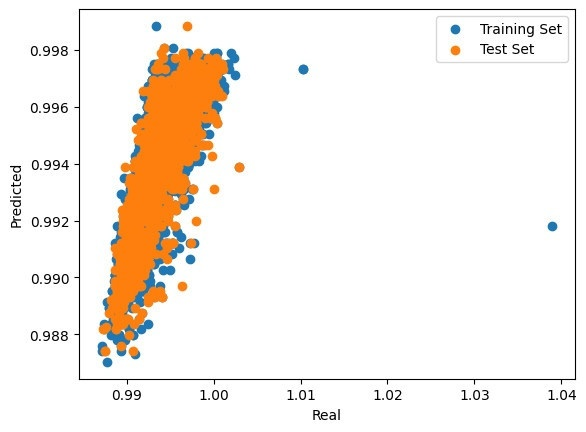
\includegraphics[width=\linewidth]{Machine_learning/images/linear_reg.jpeg}
    \caption{Linear regression plot between actual and predicted-trained data}
    %\label{fig:enter-label}
\end{figure}

\subsubsection{Multiple Linear Regression}
Multiple Linear Regression (MLR) is a generalization of classical linear regression. MLR models a linear relationship between the target response and multiple explanatory variables.

\[
y_i = \beta_0 + \beta_1 x_{i1} + \beta_2 x_{i2} + \cdots + \beta_p x_{ip}
\]
Since MLR is a generalization, the Scikit Learn library uses the same function that we used before for Linear Regression. So training and linear regression uses the same method from \cref{linear_reg}

\begin{lstlisting}[style=mypython]
from sklearn.linear_model import LinearRegression
multiple_linear_regression = LinearRegression()
multiple_linear_regression.fit(X = X_train, y = y_train)
\end{lstlisting}
Increasing the number of predictor variables leads to a better adjustment of the target so that the value of $R^2$ increases.

\begin{lstlisting}[style=mypython]
from sklearn.metrics import r2_score
pred_train_lr = multiple_linear_regression.predict(X_train)
pred_test_lr = multiple_linear_regression.predict(X_test)
print('R2 training = ', r2_score(y_train, pred_train_lr))
print('R2 test = ', r2_score(y_test, pred_test_lr))

Output:
R2 training =  0.9608334119853044
R2 test =  0.9724221101555639
\end{lstlisting}

\subsubsection{Root Mean Squared Error (RMSE)}

Another useful metric is Root Mean Squared Error (RMSE). It has the advantage that it can be used for non-linear models.

\[
\text{RMSE} = \sqrt{ \frac{1}{n} \sum_{i=1}^{n} (y_i - \hat{y}_i)^2 }
\]

\begin{lstlisting}[style=mypython]
from sklearn.metrics import mean_squared_error
rmse_test = np.sqrt(mean_squared_error(y_test,pred_test_lr))
print('RSME test= ', rmse_test)

Output:
RSME test=  0.00047624213322229874
\end{lstlisting}

\subsection{LASSO(Least Absolute Shrinkage and Selection Operator)}
Least Absolute Shrinkage and Selection Operator (LASSO) is a linear regression method that performs variable selection and regularization to improve prediction accuracy and produce a simpler model. This method uses a cost function with a constant $\alpha$ that determines the degree of penalization. Scikit-learn has implemented LASSO in the function \texttt{sklearn.linear\_model.Lasso}.

\[
\text{LASSO}_{\text{Cost\;Function}} = \sum_{i=1}^M (y_i - \hat{y}_i)^2 = \sum_{i=1}^M \left( y_i - \sum_{j=0}^p w_j x_{ij} \right)^2 + \alpha \sum_{j=0}^p |w_j|
\]
\[
\text{For some } t > 0, \quad \sum_{j=0}^p |w_j| < t
\]
\begin{lstlisting}[style=mypython]
from sklearn.linear_model import Lasso
lasso_regression = Lasso(alpha=0.0001)
lasso_regression.fit(X = X_train, y = y_train)
\end{lstlisting}

\begin{lstlisting}[style=mypython]
from sklearn.metrics import r2_score, mean_squared_error
y_pred = lasso_regression.predict(X_test)
r2 = r2_score(y_test, y_pred)
print('R2 test = ', r2)

Output:
R2 test =  0.9680058702120279
\end{lstlisting}
Let's analyze if using LASSO we have a smaller model where some of the coefficients are zero.
\begin{lstlisting}[style=mypython]
coeffecients = pd.DataFrame(lasso_regression.coef_,X.columns.tolist())
coeffecients.columns = ['Coeffecient']
print(coeffecients)

Output:
                      Coeffecient
fixed acidity            0.000518
volatile acidity         0.000000
citric acid              0.000000
residual sugar           0.001855
chlorides                0.000027
free sulfur dioxide     -0.000000
total sulfur dioxide     0.000090
pH                       0.000345
sulphates                0.000096
alcohol                 -0.001337
\end{lstlisting}

\begin{lstlisting}[style=mypython]
coefficients.plot.bar()
\end{lstlisting}
\begin{figure}[H]
    \centering
    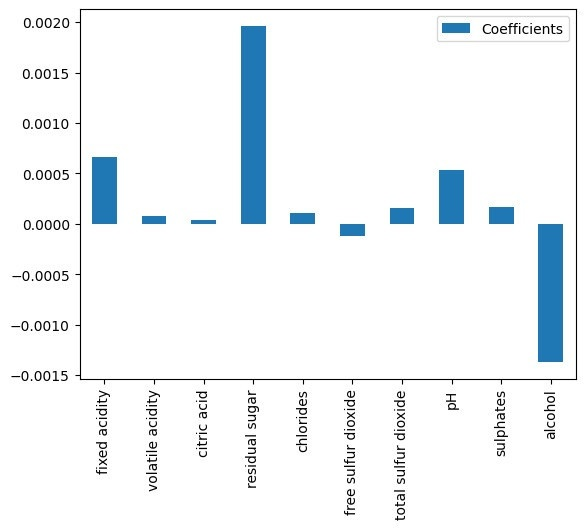
\includegraphics[width=0.5\linewidth]{Machine_learning/images/lasso_bar.jpeg}
    \caption{Bar plot of coefficients analyzed using LASSO}
    %\label{fig:enter-label}
\end{figure}
Finally, we will analyze how the RSME of the training and test sets change for different alpha values.

\begin{lstlisting}[style=mypython]
alphas=np.logspace(-10,3,endpoint=True,num=100,base=10)
RMSE=[]
RMSE_p=[]
for x in (alphas):
    #print(x)
    model_lasso = Lasso(x)
    model_lasso.fit(X_train, y_train)
    pred_test_lasso= model_lasso.predict(X_test)
    pred_train_lasso=model_lasso.predict(X_train)
    RMSE_p.append(np.sqrt(mean_squared_error(y_test,pred_test_lasso)))
    RMSE.append(np.sqrt(mean_squared_error(y_train,pred_train_lasso)))
fig=plt.gcf()
fig.set_size_inches(12,7)
plt.plot(alphas,RMSE, label='Training Set', linewidth=6)
plt.plot(alphas,RMSE_p, label='Test Set',linewidth=6)
plt.plot(alphas,len(alphas)*[rmse_MLR], label='MLR',linewidth=4)
plt.xscale("log")
plt.xlabel('alpha')
plt.ylabel('RMSE')
plt.legend()
\end{lstlisting}

\begin{figure}[H]
    \centering
    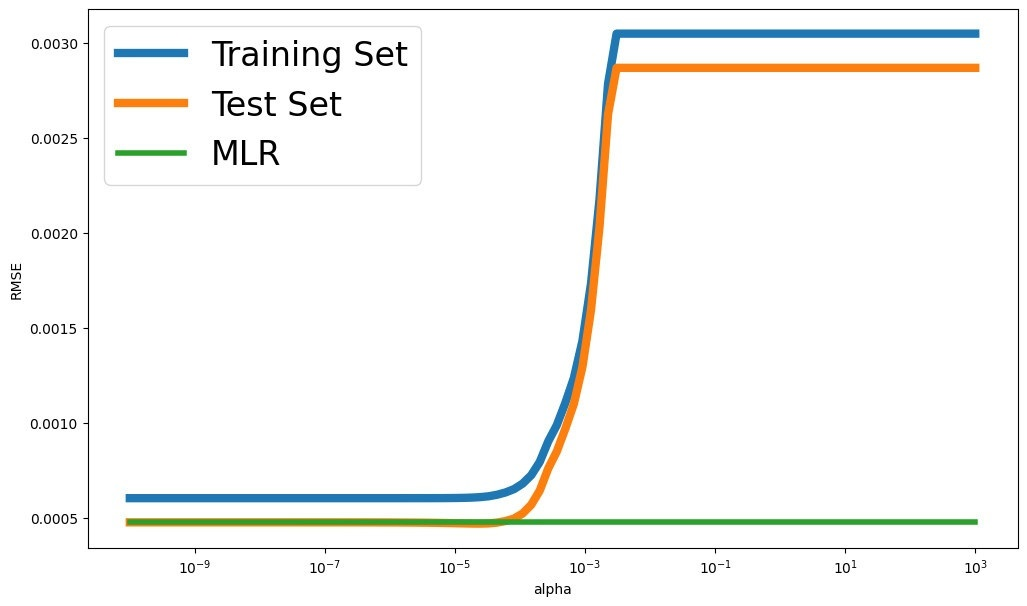
\includegraphics[width=\linewidth]{Machine_learning/images/lasso.jpeg}
    \caption{Bar plot of coefficients analyzed using LASSO}
    %\label{fig:enter-label}
\end{figure}

%\subsection{Application: Prediction of Density}

\subsection{Discussion and Conclusion}
From the analysis of red $\&$ white wine-quality dataset. We can conclude these difference between red and white wine - Red wines exhibit higher levels of volatile acidity, sulphates $\&$ chlorides content, and density. In contrast, white wines show significantly higher residual sugar and sulfur dioxide content which indicates a sweeter and more preserved character. Additionally, white wines tend to have slightly higher average quality ratings, possibly due to their cleaner fermentation and lower acidity.

This study demonstrates that machine learning is a powerful tool for chemists, enabling efficient analysis, visualization, and interpretation of experimental data. Through hands-on work with five Python notebooks, covering topics from classification and regression to data visualization, participants applied ML techniques to a real-world wine dataset.

The project shows that even small datasets can benefit from data-driven approaches, as illustrated in \cref{project2section} Integrating machine learning into chemical research enhances data handling and supports better scientific conclusions. Overall, ML is becoming an essential skill for chemists, streamlining research and accelerating discovery.\\

\noindent\dotfill



\newpage
\section*{Appendix}
\addcontentsline{toc}{section}{Appendix}
\begin{enumerate}
    \item \href{https://pubs.acs.org/doi/suppl/10.1021/ed082p953/suppl_file/jce2005p0953w.pdf}{Supplementary material of project 1 containing theatrical data used for calculating percentage error.}
    \item \href{https://archive.ics.uci.edu/dataset/186/wine+quality}{Red and White wine-quality dataset. }
    \item \href{https://docs.google.com/spreadsheets/d/1YVUVZeZ_wiyl1l1sGVrfcRbrWC0P5ydPrFI7W2mUbzQ/edit?usp=sharing}{$1^{st}$ experiment-Aromaticity dataset Google-sheets}
    \item \href{https://docs.google.com/spreadsheets/d/1DhclPD_BuQI6k3KOSAlNELtijxsx-F_Mzil6ODMJ_lI/edit?usp=sharing}{$2^{nd}$ experiment-Acid Base Dataset Google-Sheets}
    \item \href{https://github.com/jeevakathirvel11/Summer_Internship}{Computational chemistry github}. Molecule construction, input $\&$ output files of $1^{st}$ and $2^{nd}$.
    \item \href{https://github.com/jeevakathirvel11/Intro-to-Machine-Learning-in-Chemistry.git}{Machine Learning for chemist}. $3^{rd}$ experiment's worked-out Assignments and Jupyter Notebooks.
    \item \href{https://drive.google.com/drive/folders/1kaaZYR6s1578xgS4SVJjO0Ni_yRnoT6p?usp=sharing}{Google-colab Interactive Python Notebooks}
    \item \href{https://in.mirrors.cicku.me/ctan/macros/latex/contrib/mhchem/mhchem.pdf}{\textit{\textbf{mhchem}} Chemistry Equation \LaTeX package}. Chemical equations in the report used this package.
    \item \href{https://mirror.niser.ac.in/ctan/macros/generic/chemfig/chemfig-en.pdf}{\textit{\textbf{chemfig}} Chemistry structures drawing \LaTeX package. Cyclic Organic Chemical figures in this report are build using this package.}
\end{enumerate}


\bibliographystyle{plain}
\bibliography{Reference}

\noindent\dotfill


\end{document}



